\begin{enumerate}[label={},font=\normalfont,leftmargin=1.15cm,labelwidth=1.0cm,labelsep=0.15cm,itemindent=0pt,listparindent=0pt,parsep=0pt,topsep=0pt]
\item[1.2.1] The roots of the quadratic equation $(x-1)^2=16$ are:

\begin{multicols}{4}
\begin{enumerate}
\setlength{\itemsep}{0pt}
    \item $5,3$
    \item $4,-4$
    \item $5,-3$
    \item $-5,3$\nobreak\hfill\mbox{(10,2026)}
\end{enumerate}
\end{multicols}



\vspace{0.6em}\par\solution

Set $f(x)=(x-1)^2-16$. The required roots satisfy $f(x)=0$, and $f'(x)=2(x-1)$. Newton--Raphson gives
\[
x_{n+1}=x_n-\frac{(x_n-1)^2-16}{2(x_n-1)},\qquad x_n\ne1.
\]
\par\noindent\hfill\mbox{\textit{(\ref{formula-1-1-11})}}\par
Starting from $x_0=0$ and $x_0=6$ gives the following iterates:
\[
\begin{array}{c|r|r}
n & x_n\;(x_0=0) & x_n\;(x_0=6)\\\hline
0 & 0.000000 & 6.000000\\
1 & -7.500000 & 5.100000\\
2 & -4.191176 & 5.001220\\
3 & -3.136665 & 5.000000\\
4 & -3.002258 & 5.000000\\
5 & -3.000001 & 5.000000\\
6 & -3.000000 & 5.000000
\end{array}
\]
Factorization independently confirms the result:
\[
(x-1)^2-16=((x-1)-4)((x-1)+4)=(x-5)(x+3)=0.
\]
Hence the exact roots are $5$ and $-3$. Substitution verifies $(5-1)^2=16$ and $(-3-1)^2=16$. These agree with the Newton--Raphson limits, while the residuals $f(x_n)$ tend to zero; therefore the iteration has found both roots. The correct answer is \textbf{c)}.

The C program prints the Newton--Raphson iterates for both starting values and returns the two roots:
\begin{lstlisting}[frame=single, basicstyle=\rmfamily, escapeinside={(*@}{@*)}]
(*@\makebox[\dimexpr\linewidth-2\fboxsep-2\fboxrule\relax][c]{codes/1.2.1.c}@*)
\end{lstlisting}
The Python program plots the two curves and marks their intersections:
\begin{lstlisting}[frame=single, basicstyle=\rmfamily, escapeinside={(*@}{@*)}]
(*@\makebox[\dimexpr\linewidth-2\fboxsep-2\fboxrule\relax][c]{codes/1.2.1.py}@*)
\end{lstlisting}
\begin{figure}[H]
    \centering
    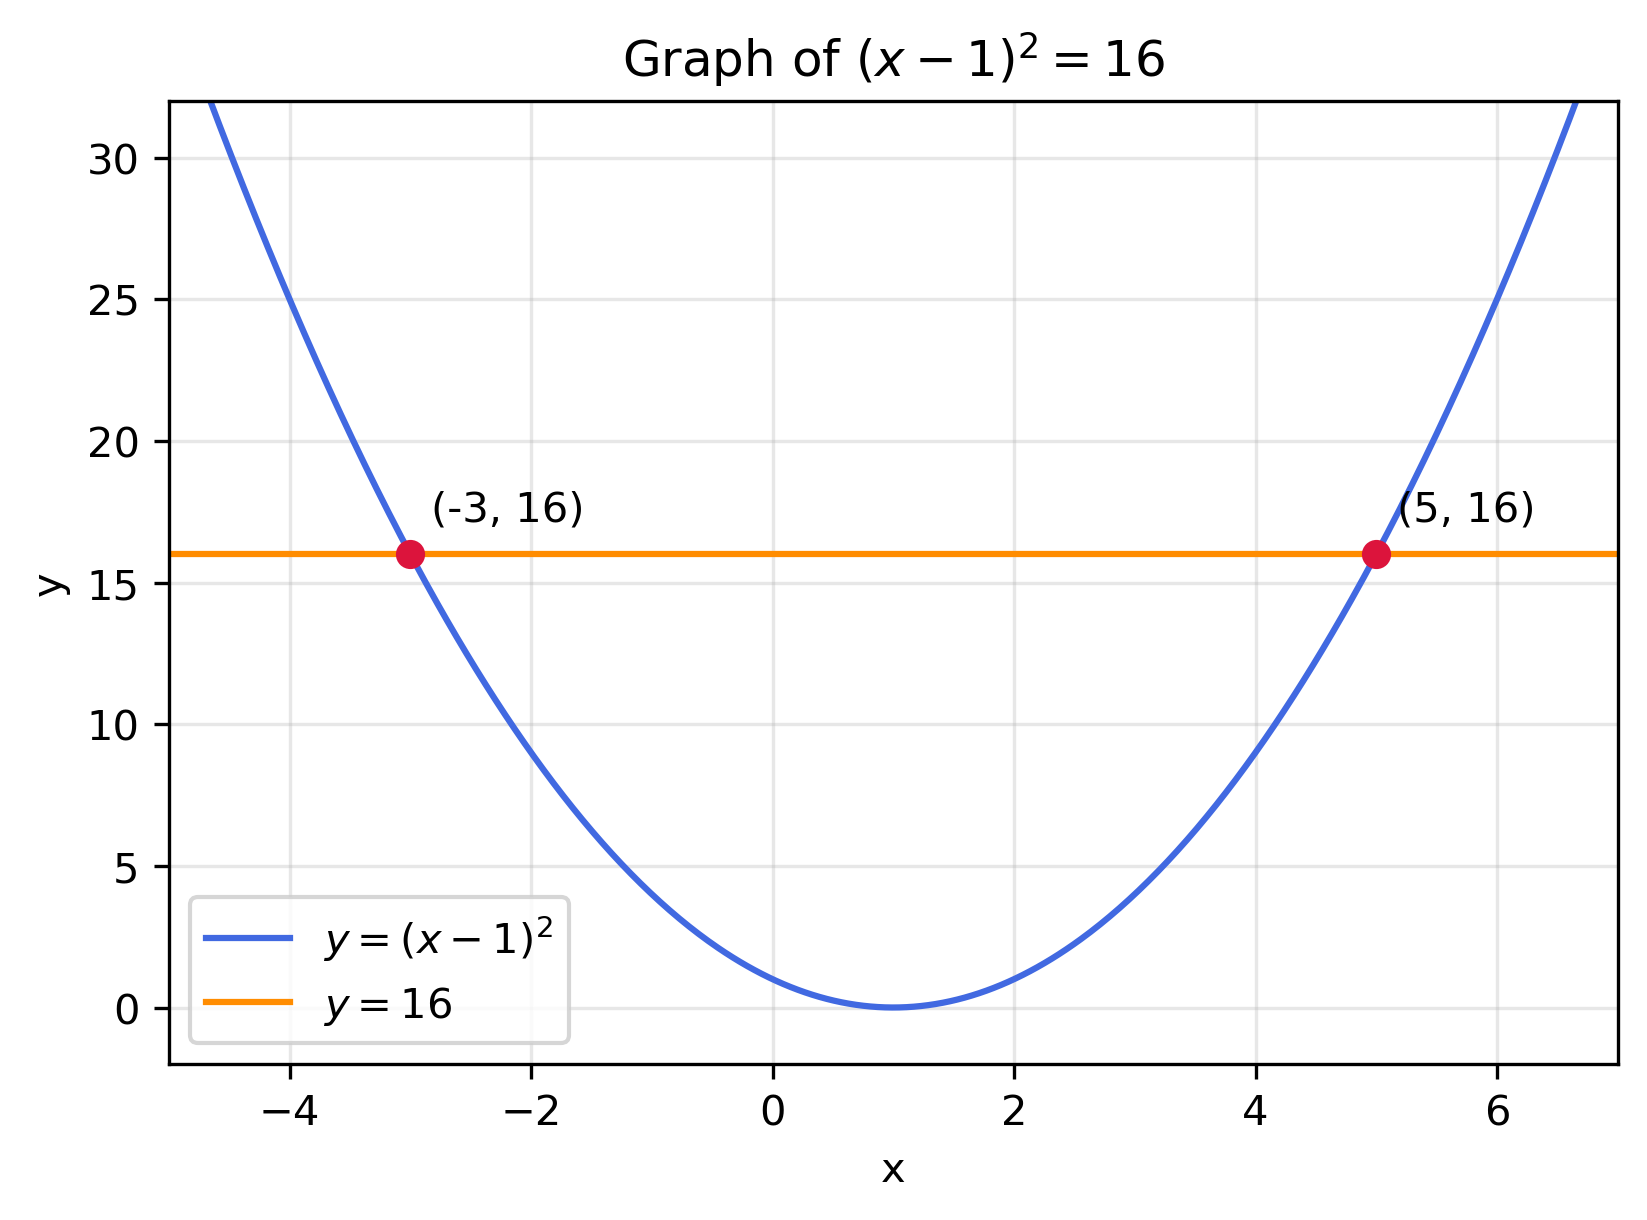
\includegraphics[width=0.48\linewidth]{figs/1.2.1.png}
    \caption{Intersections of $y=(x-1)^2$ and $y=16$, corresponding to roots $x=-3$ and $x=5$.}
\end{figure}

\item[1.2.2] In the figure, $PQ$ and $PR$ are tangents to a circle with centre $O$ and radius $3$ cm. If $\angle QPR=60^\circ$, find the length of each tangent.

\begin{multicols}{2}
\begin{enumerate}
\setlength{\itemsep}{0pt}
    \item $3\sqrt3$ cm
    \item $3$ cm
    \item $6$ cm
    \item $\sqrt3$ cm\nobreak\hfill\mbox{(10,2026)}
\end{enumerate}
\end{multicols}



\vspace{0.6em}\par\solution

The equal tangents make $OP$ bisect the $60^\circ$ angle, so $\angle QPO=30^\circ$. In right triangle $OQP$, $OP=OQ/\sin30^\circ=6$ cm. Let $\mathbf o,\mathbf p,\mathbf q,\mathbf r$ be the position vectors of the actual points, and define $\mathbf u=\mathbf p-\mathbf o$, $\mathbf v=\mathbf q-\mathbf o$, and $\mathbf w=\mathbf r-\mathbf o$. Then $\mathbf u^T\mathbf u=36$ and $\mathbf v^T\mathbf v=\mathbf w^T\mathbf w=9$. Radius-tangent perpendicularity gives
\[
\mathbf v^T(\mathbf u-\mathbf v)=0,\qquad
\mathbf w^T(\mathbf u-\mathbf w)=0,
\]
so $\mathbf u^T\mathbf v=\mathbf u^T\mathbf w=9$. Therefore
\[
\begin{aligned}
PQ^2&=(\mathbf u-\mathbf v)^T(\mathbf u-\mathbf v)=36-18+9=27,\\
PR^2&=(\mathbf u-\mathbf w)^T(\mathbf u-\mathbf w)=36-18+9=27.
\end{aligned}
\]
Hence $PQ=PR=\sqrt{27}=3\sqrt3$ cm.
\par\noindent\hfill\mbox{\textit{(\ref{formula-1-1-2})}}\par
As a consistency check, $\angle QOR=120^\circ$; hence $\mathbf v^T\mathbf w=9\cos120^\circ=-9/2$. Thus $(\mathbf q-\mathbf p)^T(\mathbf r-\mathbf p)=27/2$, and dividing by $PQ\,PR=27$ gives $\cos\angle QPR=1/2$. The given angle is satisfied, and the answer is \textbf{a)}.

The C program checks the radius, perpendicularity, equal tangent lengths and angle using vector products:
\begin{lstlisting}[frame=single, basicstyle=\rmfamily, escapeinside={(*@}{@*)}]
(*@\makebox[\dimexpr\linewidth-2\fboxsep-2\fboxrule\relax][c]{codes/1.2.2.c}@*)
\end{lstlisting}
The Python program draws the construction from the four points $O,P,Q,R$, using CoordGeo to generate the circle and line segments:
\begin{lstlisting}[frame=single, basicstyle=\rmfamily, escapeinside={(*@}{@*)}]
(*@\makebox[\dimexpr\linewidth-2\fboxsep-2\fboxrule\relax][c]{codes/1.2.2.py}@*)
\end{lstlisting}
\begin{figure}[H]
    \centering
    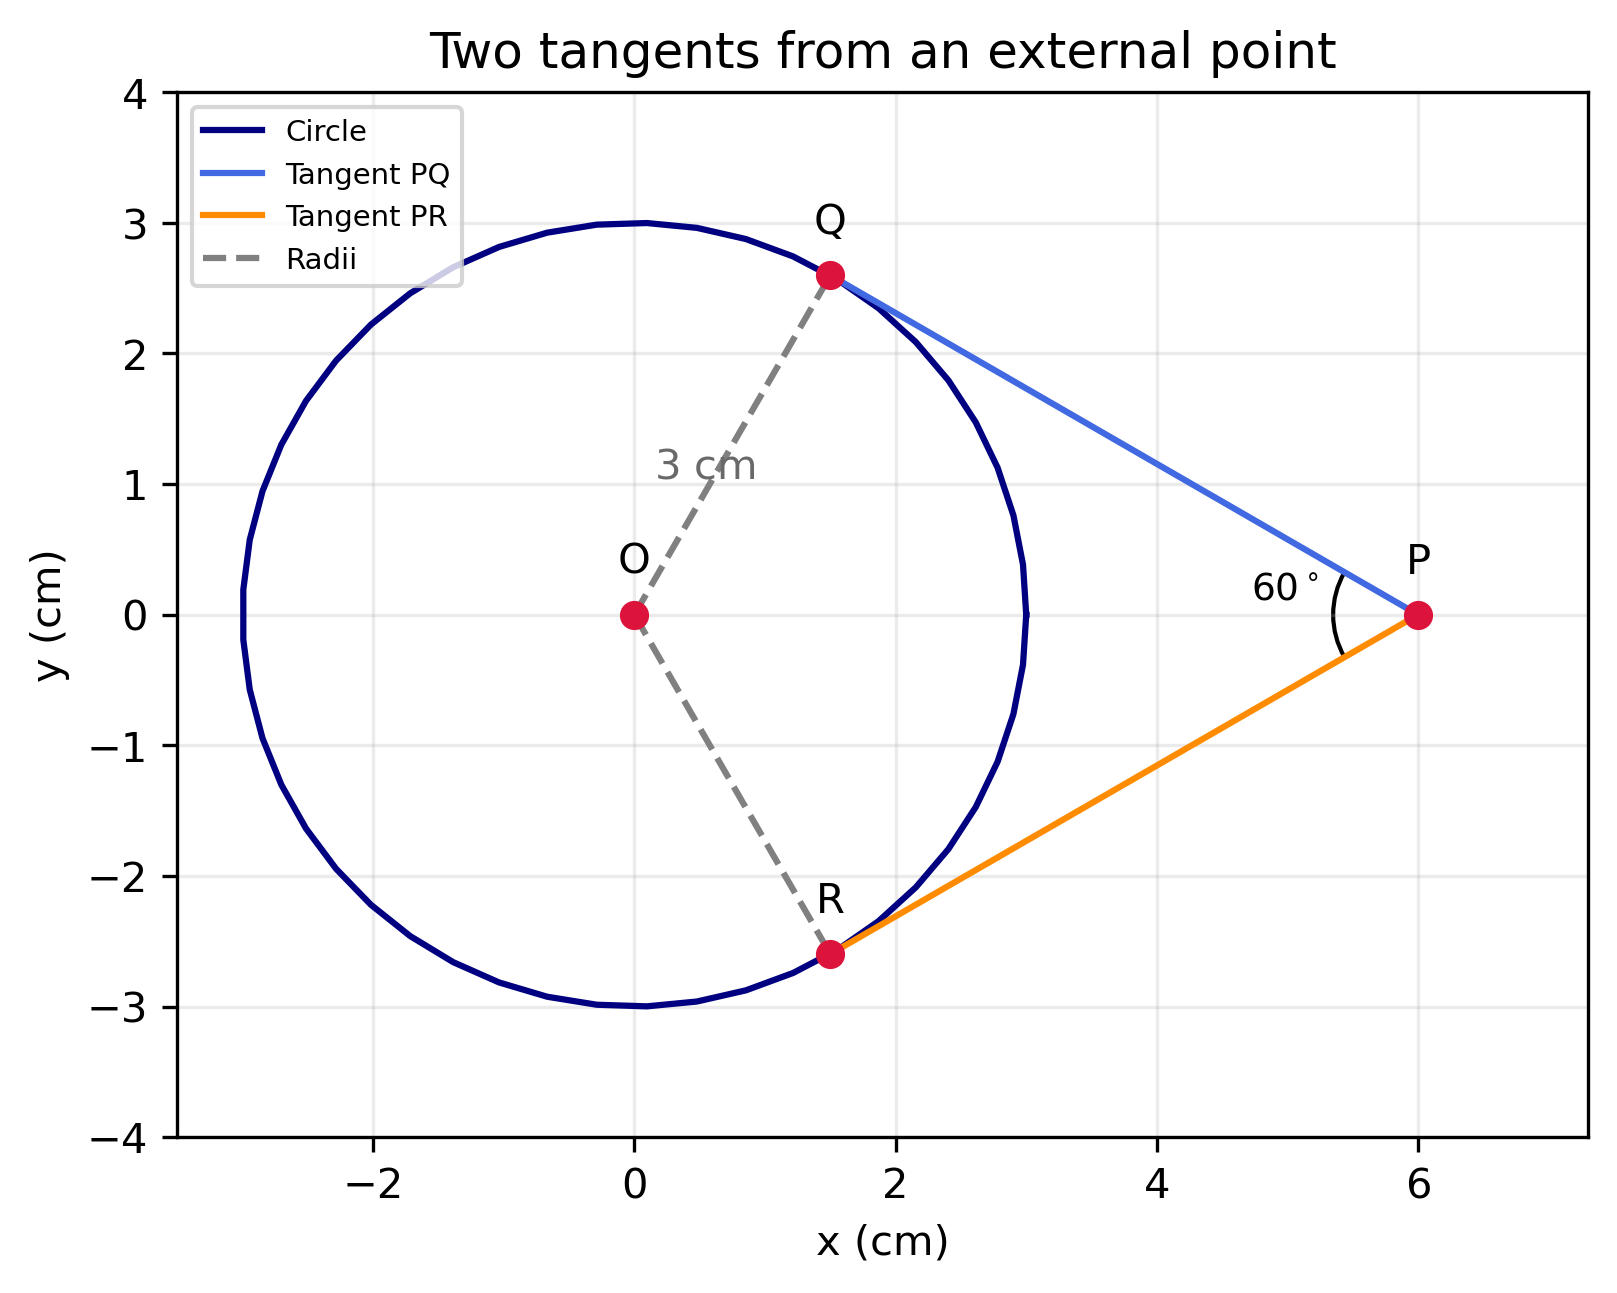
\includegraphics[width=0.47\linewidth]{figs/1.2.2.png}
    \caption{Circle with centre $O$, external point $P$, and tangent points $Q$ and $R$.}
\end{figure}

\item[1.2.3] The number $(3\times11\times13+3)$ is:

\begin{multicols}{4}
\begin{enumerate}
\setlength{\itemsep}{0pt}
    \item prime
    \item divisible by $13$
    \item composite
    \item odd\nobreak\hfill\mbox{(10,2026)}
\end{enumerate}
\end{multicols}



\vspace{0.6em}\par\solution

The following code verifies each option.
\begin{lstlisting}[frame=single, basicstyle=\rmfamily, escapeinside={(*@}{@*)}]
(*@\makebox[\dimexpr\linewidth-2\fboxsep-2\fboxrule\relax][c]{codes/1.2.3.c}@*)
\end{lstlisting}

\item[1.2.4] Two dice are rolled together. Find the probability that the sum of the numbers obtained is divisible by $6$.

\begin{multicols}{4}
\begin{enumerate}
\setlength{\itemsep}{0pt}
    \item $\frac16$
    \item $\frac{11}{36}$
    \item $\frac1{12}$
    \item $\frac14$\nobreak\hfill\mbox{(10,2026)}
\end{enumerate}
\end{multicols}



\vspace{0.6em}\par\solution


Each die can show $1$ through $6$, giving $36$ equally likely ordered pairs. For sums $2\le s\le7$, there are $s-1$ pairs, from $(1,s-1)$ through $(s-1,1)$. For sums $8\le s\le12$, the first die can show $s-6$ through $6$, giving $13-s$ pairs. Dividing these counts by $36$ gives the PMF:
\[
p_S(s)=P(S=s)=\begin{cases}
\dfrac{s-1}{36},&2\le s\le7,\\[6pt]
\dfrac{13-s}{36},&8\le s\le12,\\[6pt]
0,&\text{otherwise}.
\end{cases}
\]
The sum is divisible by $6$ only for $S=6$ and $S=12$. Therefore, using the PMF,
\[
P(S\text{ is divisible by }6)=P(S=6)+P(S=12)=\frac5{36}+\frac1{36}=\boxed{\frac16},
\]
option \textbf{a)}. The Python code uses NumPy's random number generator to simulate dice rolls and plots the simulated PMF alongside the exact PMF.
\par\noindent\hfill\mbox{\textit{(\ref{formula-1-1-9})}}\par\begin{lstlisting}[frame=single, basicstyle=\rmfamily, escapeinside={(*@}{@*)}]
(*@\makebox[\dimexpr\linewidth-2\fboxsep-2\fboxrule\relax][c]{codes/1.2.4.py}@*)
\end{lstlisting}
\begin{figure}[H]
    \centering
    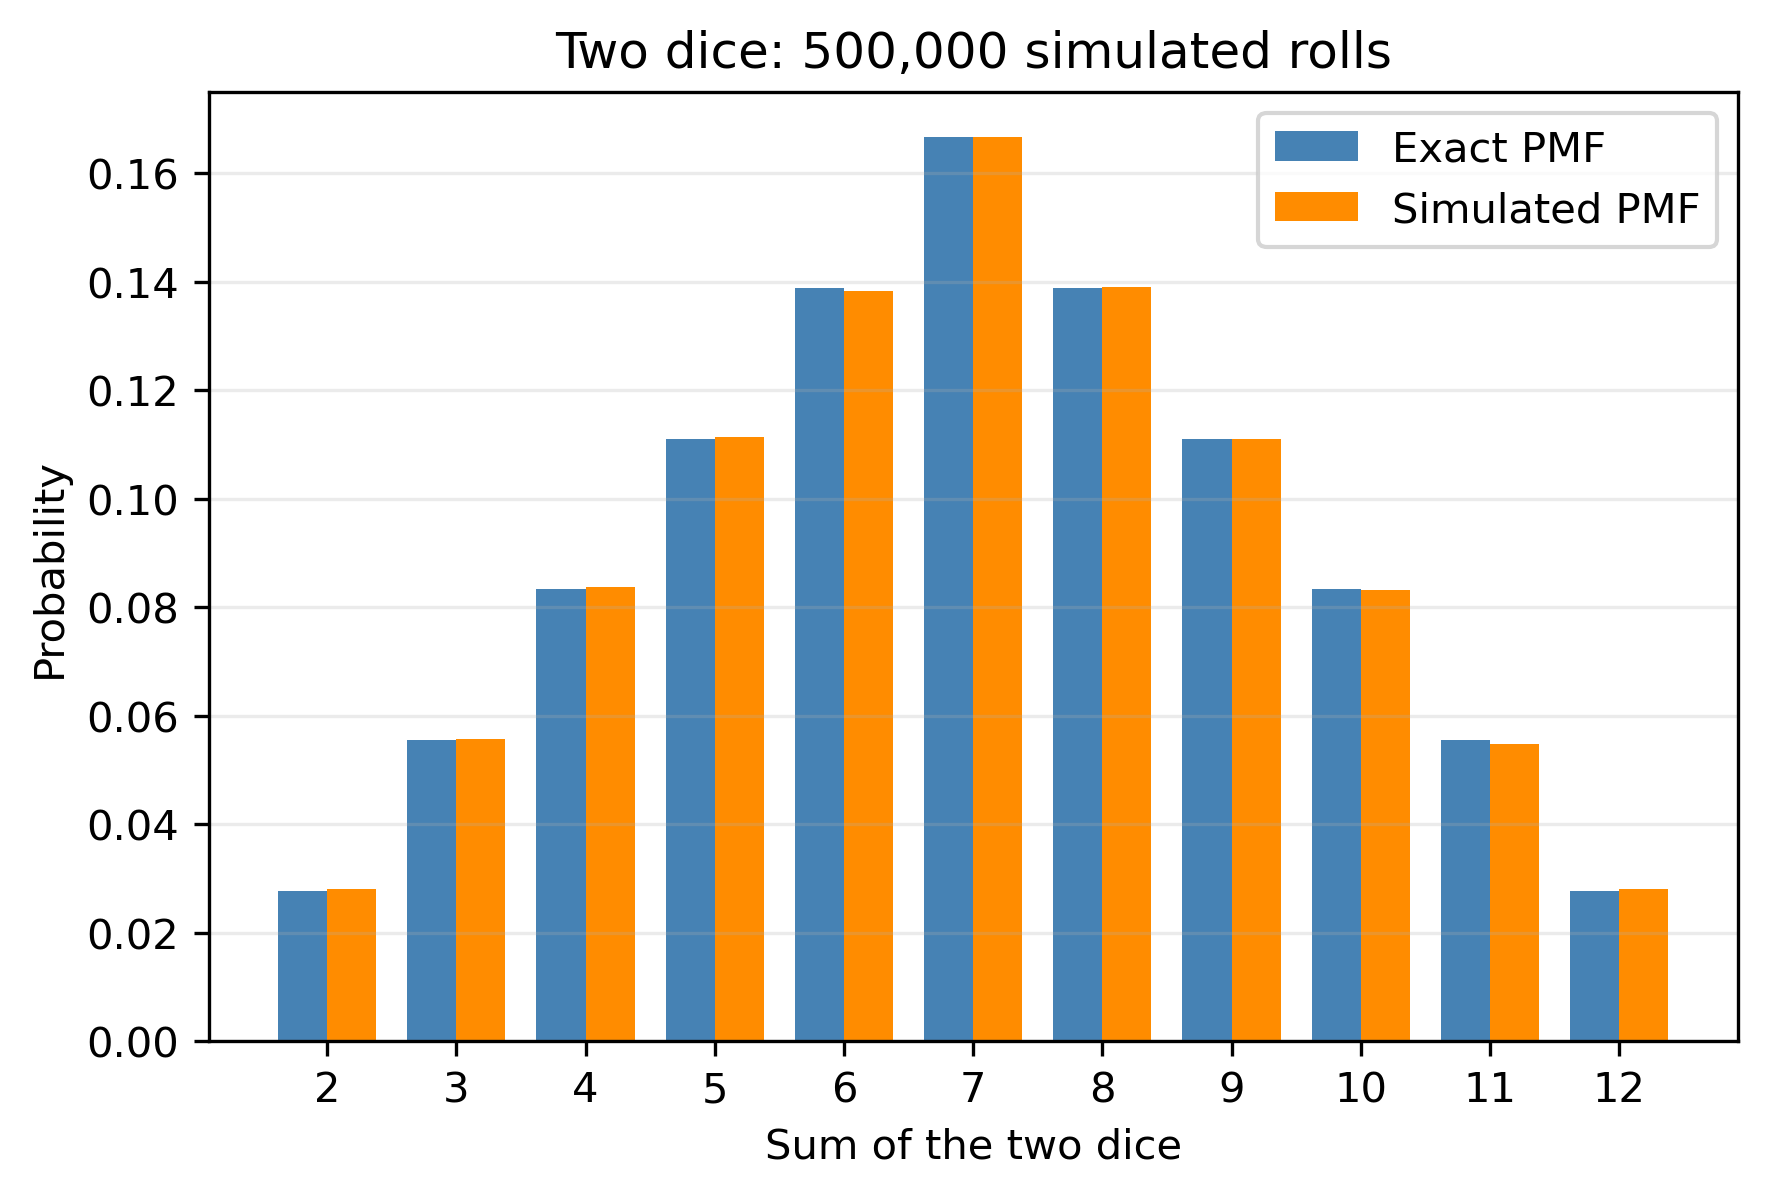
\includegraphics[width=0.50\linewidth]{figs/1.2.4.png}
    \caption{Simulated and exact probability distributions for the sum of two dice.}
\end{figure}

\item[1.2.5] The equation of another line parallel to $2x-6y=7$ is:

\begin{multicols}{2}
\begin{enumerate}
\setlength{\itemsep}{0pt}
    \item $y=3x-7$
    \item $2x=9-6y$
    \item $x-3y=7$
    \item $x=\frac72-3y$\nobreak\hfill\mbox{(10,2026)}
\end{enumerate}
\end{multicols}



\vspace{0.6em}\par\solution


The given line has slope $\frac13$. Only option c), $y=\frac13x-\frac73$, has the same slope and a different intercept. Hence the answer is \textbf{c)}. The code plots the given line and all four options.
\par\noindent\hfill\mbox{\textit{(\ref{formula-1-1-5})}}\par\begin{lstlisting}[frame=single, basicstyle=\rmfamily, escapeinside={(*@}{@*)}]
(*@\makebox[\dimexpr\linewidth-2\fboxsep-2\fboxrule\relax][c]{codes/1.2.5.py}@*)
\end{lstlisting}
\begin{figure}[H]
    \centering
    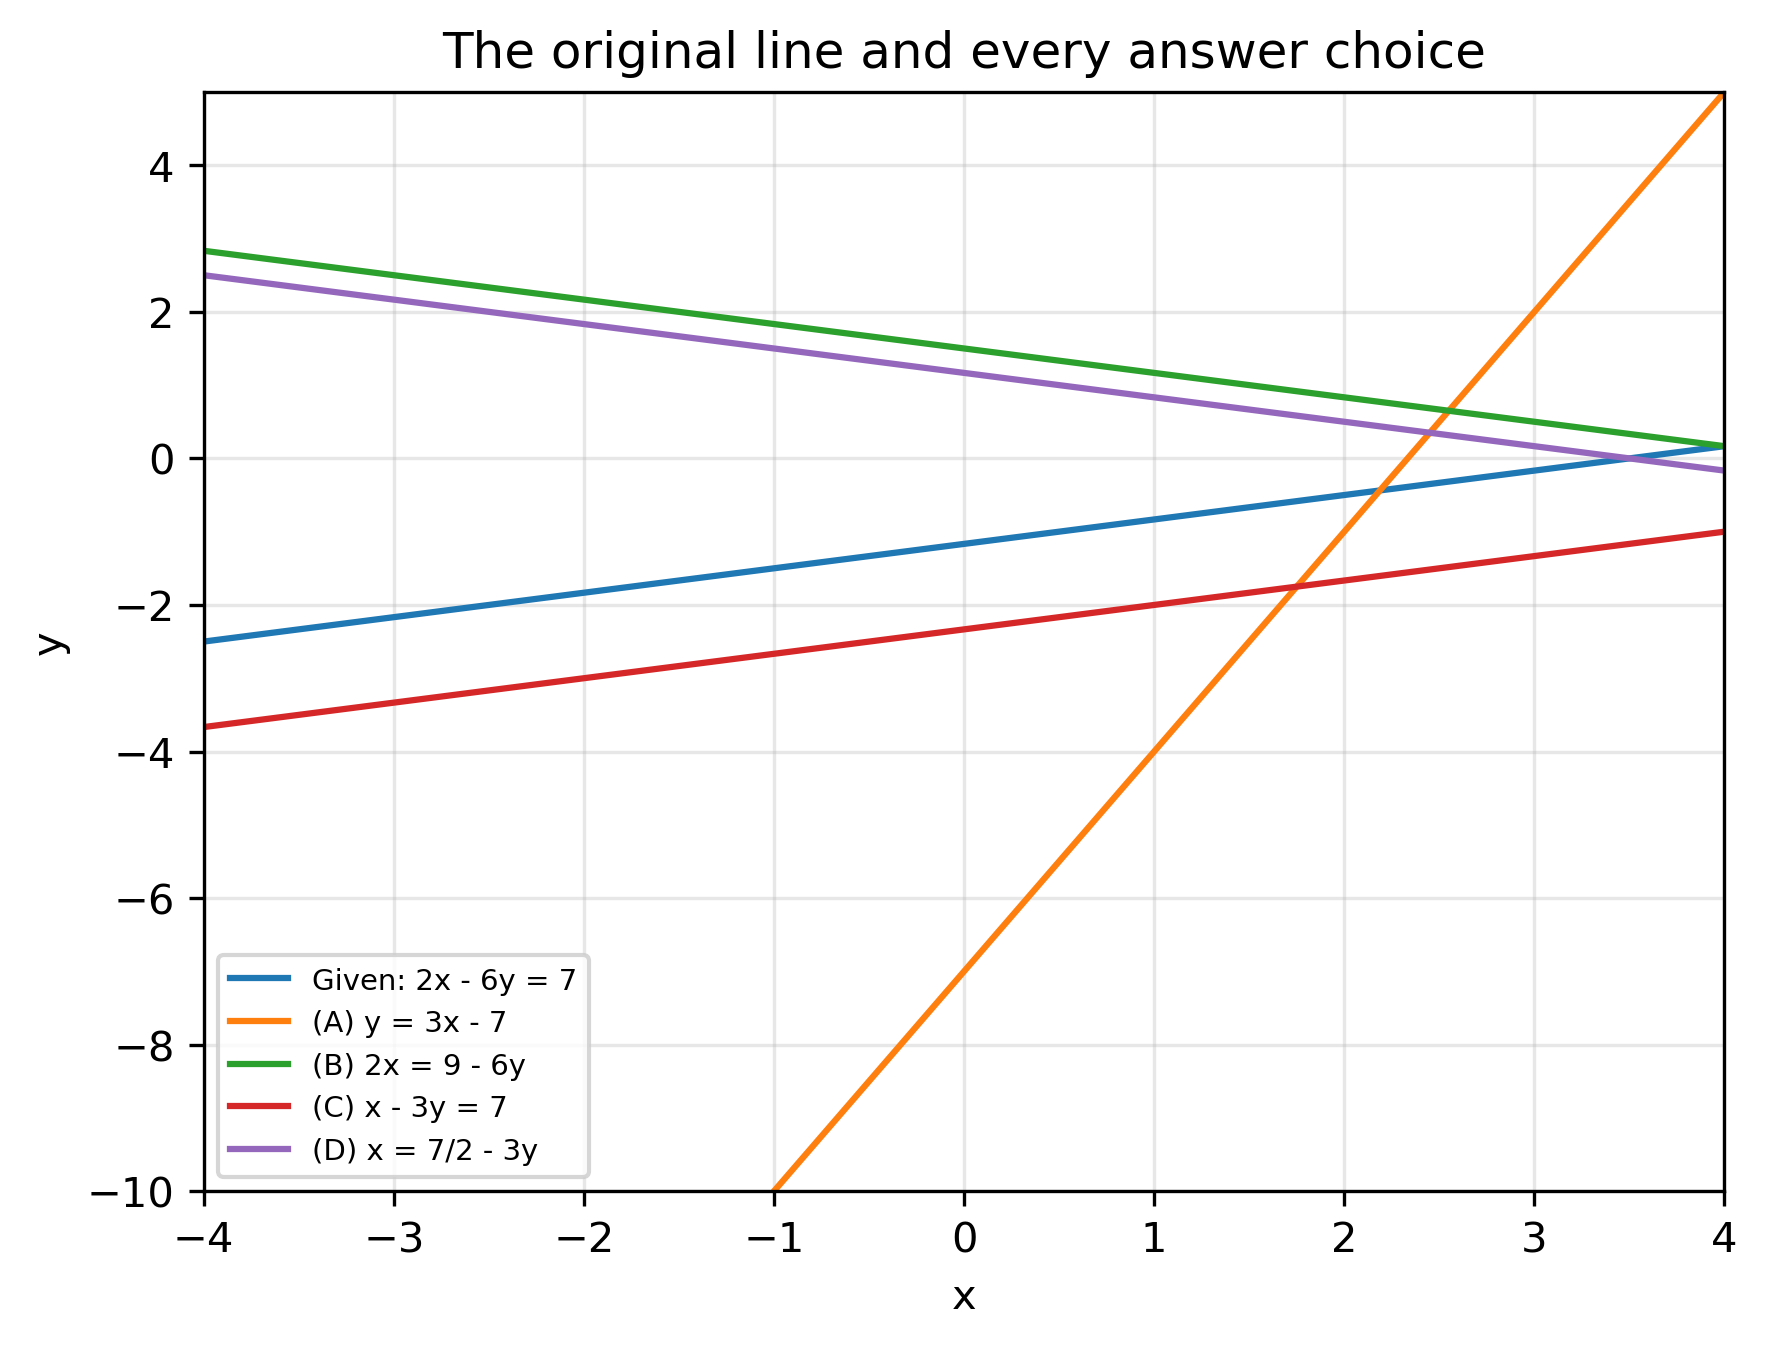
\includegraphics[width=0.52\linewidth]{figs/1.2.5.png}
    \caption{The given line and the four candidate lines.}
\end{figure}

\item[1.2.6] If the roots of $\sqrt3x^2-kx+2\sqrt3=0$ are real and equal, find the value(s) of $k$.

\begin{multicols}{4}
\begin{enumerate}
\setlength{\itemsep}{0pt}
    \item $\pm\sqrt{24}$
    \item $0$
    \item $4$
    \item $-5$\nobreak\hfill\mbox{(10,2026)}
\end{enumerate}
\end{multicols}



\vspace{0.6em}\par\solution

For $\sqrt3x^2-kx+2\sqrt3=0$, the discriminant is $D(k)=k^2-24$. Equal real roots require $D(k)=0$. Apply Newton--Raphson to $g(k)=k^2-24$, whose derivative is $g'(k)=2k$:
\[
k_{n+1}=k_n-\frac{k_n^2-24}{2k_n},\qquad k_n\ne0.
\]
\par\noindent\hfill\mbox{\textit{(\ref{formula-1-1-1}, \ref{formula-1-1-11})}}\par
Starting from $k_0=-4$ and $k_0=4$ gives
\[
\begin{array}{c|r|r}
n&k_n\;(k_0=-4)&k_n\;(k_0=4)\\\hline
0&-4.000000&4.000000\\
1&-5.000000&5.000000\\
2&-4.900000&4.900000\\
3&-4.898980&4.898980\\
4&-4.898979&4.898979
\end{array}
\]
Factorization confirms the limits: $k^2-24=(k-2\sqrt6)(k+2\sqrt6)$, so $k=\pm2\sqrt6=\pm\sqrt{24}$. Substituting these values into the original quadratic gives $\sqrt3(x-\sqrt2)^2=0$ for $k=2\sqrt6$ and $\sqrt3(x+\sqrt2)^2=0$ for $k=-2\sqrt6$. Thus each value gives a repeated real root, verifying the iteration. The correct answer is \textbf{a)}.

The C program applies Newton--Raphson from both starting values and verifies the repeated roots:
\begin{lstlisting}[frame=single, basicstyle=\rmfamily, escapeinside={(*@}{@*)}]
(*@\makebox[\dimexpr\linewidth-2\fboxsep-2\fboxrule\relax][c]{codes/1.2.6.c}@*)
\end{lstlisting}
The Python program only plots the two resulting parabolas:
\begin{lstlisting}[frame=single, basicstyle=\rmfamily, escapeinside={(*@}{@*)}]
(*@\makebox[\dimexpr\linewidth-2\fboxsep-2\fboxrule\relax][c]{codes/1.2.6.py}@*)
\end{lstlisting}
\begin{figure}[H]
    \centering
    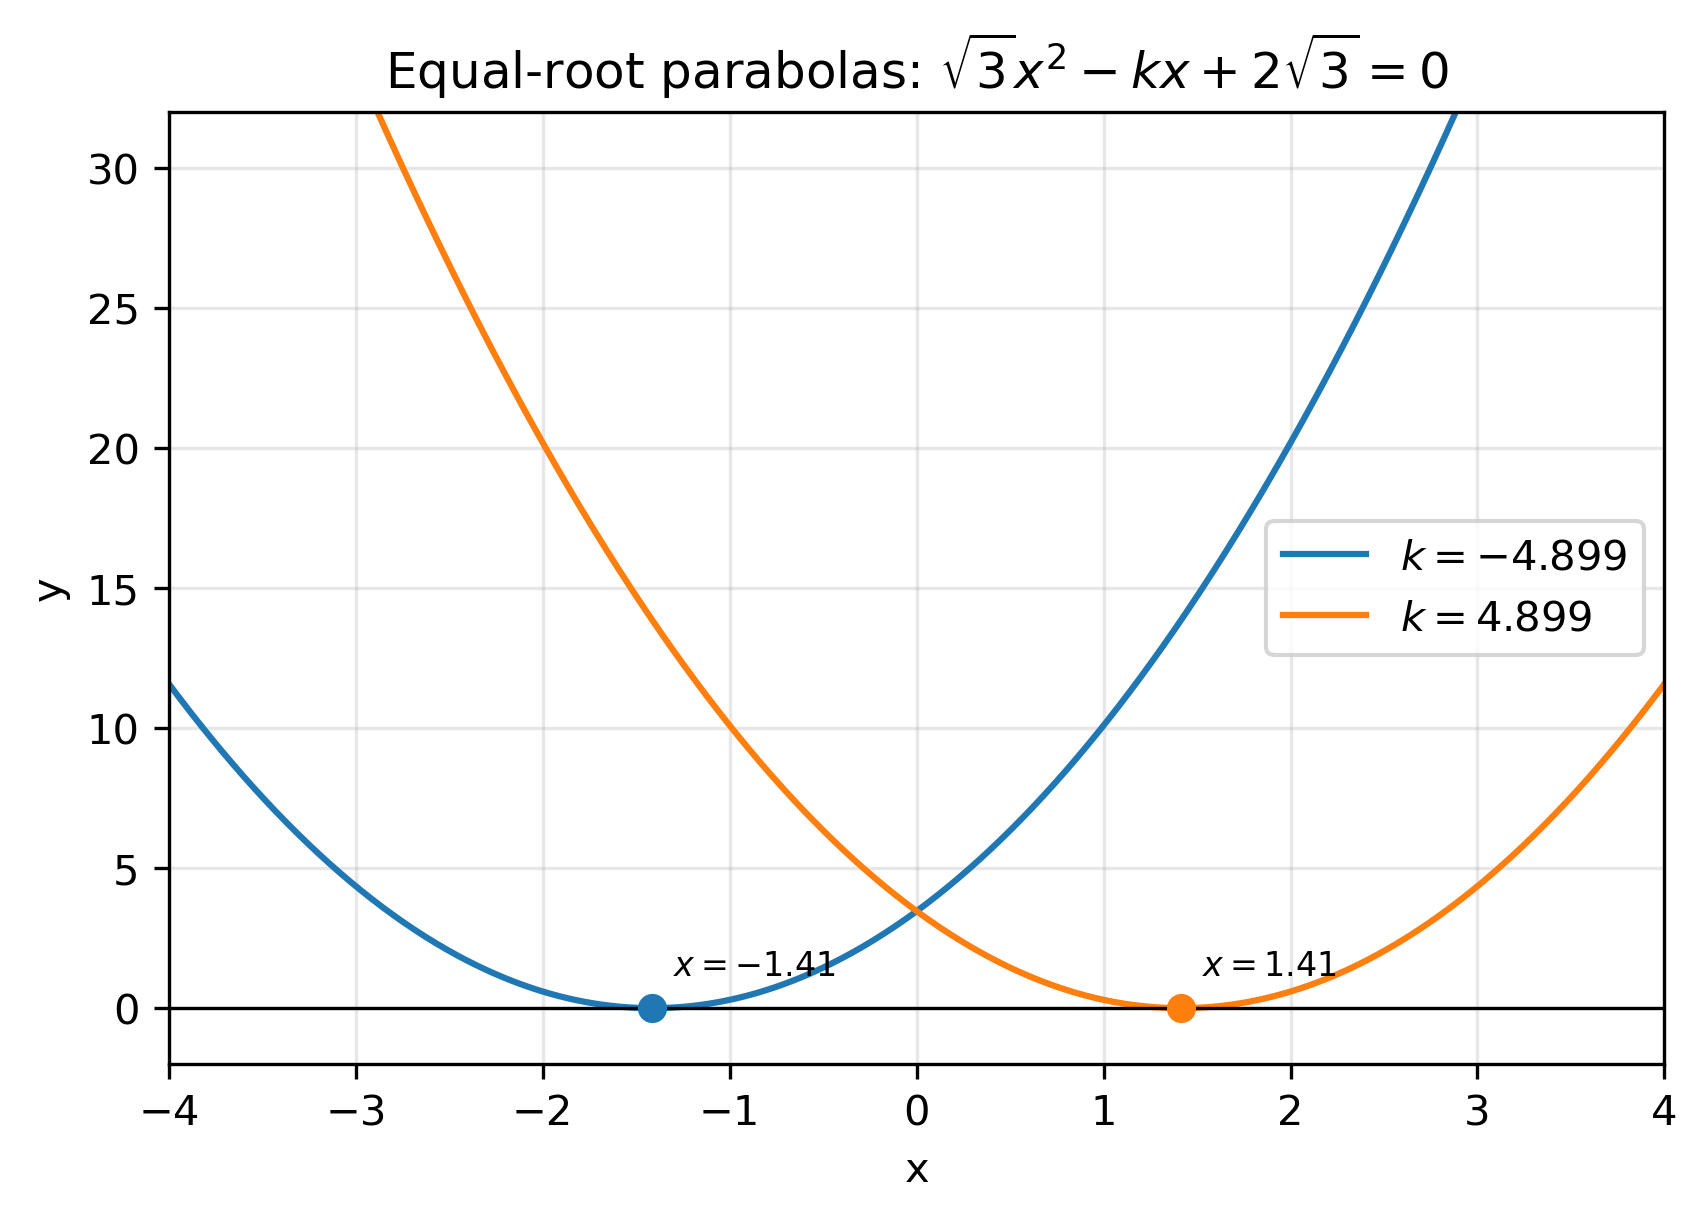
\includegraphics[width=0.52\linewidth]{figs/1.2.6.png}
    \caption{The two parabolas touching the $x$-axis at their repeated roots.}
\end{figure}

\item[1.2.7] A tangent $PT$ is drawn to a circle with centre $O$ and radius $r$. If $\angle POT=45^\circ$, find $OP$.

\begin{multicols}{4}
\begin{enumerate}
\setlength{\itemsep}{0pt}
    \item $r\sqrt2$
    \item $\sqrt{2r}$
    \item $2r$
    \item $r^2$\nobreak\hfill\mbox{(10,2026)}
\end{enumerate}
\end{multicols}



\vspace{0.6em}\par\solution


Since $OT\perp PT$, $\triangle OTP$ is right-angled at $T$. With $\angle POT=45^\circ$, it is a $45^\circ$-$45^\circ$-$90^\circ$ triangle, so $OP=r\sqrt2$. The answer is \textbf{a)}. The code draws the circle, tangent, and radius and calculates $OP$.
\par\noindent\hfill\mbox{\textit{(\ref{formula-1-1-2}, \ref{formula-1-1-7})}}\par\begin{lstlisting}[frame=single, basicstyle=\rmfamily, escapeinside={(*@}{@*)}]
(*@\makebox[\dimexpr\linewidth-2\fboxsep-2\fboxrule\relax][c]{codes/1.2.7.py}@*)
\end{lstlisting}
\begin{figure}[H]
    \centering
    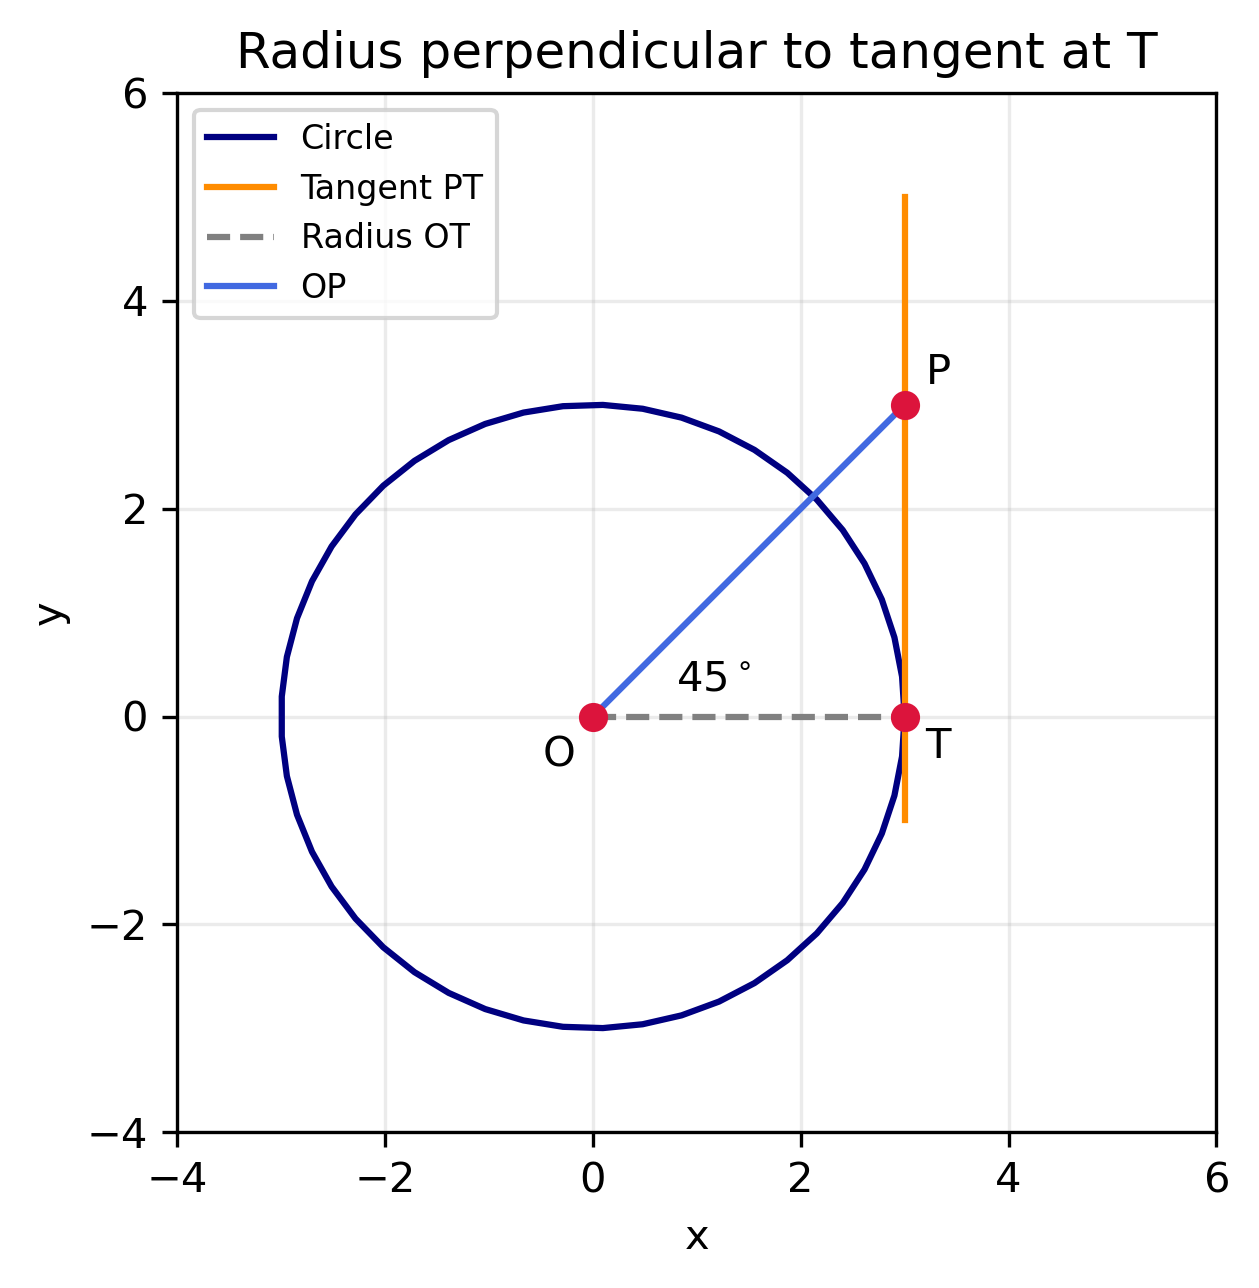
\includegraphics[width=0.48\linewidth]{figs/1.2.7.png}
    \caption{Tangent $PT$ perpendicular to radius $OT$.}
\end{figure}

\item[1.2.8] The sum and product of the zeroes of a quadratic polynomial $p(x)$ are $-\frac13$ and $2$ respectively. The polynomial $p(x)$ is:

\begin{multicols}{2}
\begin{enumerate}
\setlength{\itemsep}{0pt}
    \item $3x^2-x+6$
    \item $x^2+\frac13x-2$
    \item $3x^2-x+2$
    \item $-3x^2-x-6$\nobreak\hfill\mbox{(10,2026)}
\end{enumerate}
\end{multicols}



\vspace{0.6em}\par\solution

For $ax^2+bx+c$, the sum and product of zeroes are $-b/a$ and $c/a$. Option d) gives $-1/3$ and $2$, so it is correct. Its graph has no real zeroes, consistent with its negative discriminant.
\par\noindent\hfill\mbox{\textit{(\ref{formula-1-1-1})}}\par
The C program finds both roots by Newton--Raphson and checks their sum and product:
\begin{lstlisting}[frame=single, basicstyle=\rmfamily, escapeinside={(*@}{@*)}]
(*@\makebox[\dimexpr\linewidth-2\fboxsep-2\fboxrule\relax][c]{codes/1.2.8.c}@*)
\end{lstlisting}
The Python program only plots the selected polynomial:
\begin{lstlisting}[frame=single, basicstyle=\rmfamily, escapeinside={(*@}{@*)}]
(*@\makebox[\dimexpr\linewidth-2\fboxsep-2\fboxrule\relax][c]{codes/1.2.8.py}@*)
\end{lstlisting}
\begin{figure}[H]
    \centering
    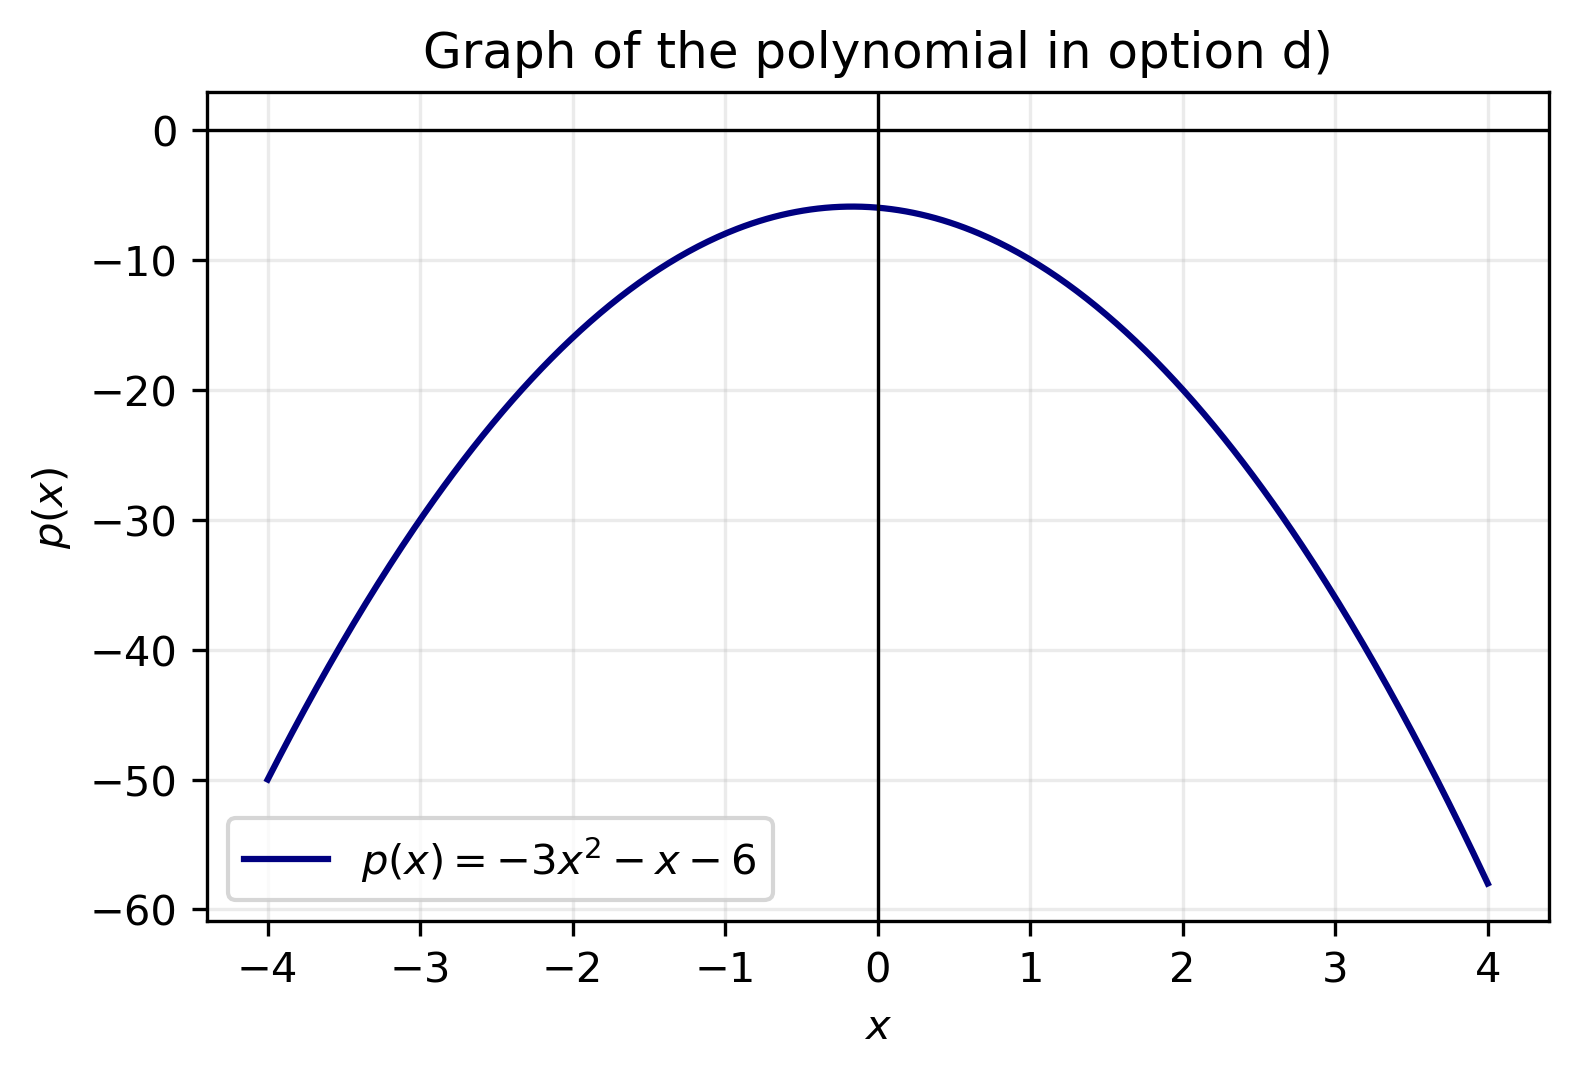
\includegraphics[width=0.51\linewidth]{figs/1.2.8.png}
    \caption{Graph of option d), which has no real zeroes.}
\end{figure}

\item[1.2.9] Find the length of a plank that can measure $4$ m $20$ cm and $5$ m $4$ cm exactly, in the least time.\nobreak\hfill\mbox{(10,2026)}



\vspace{0.6em}\par\solution


Convert the lengths to $420$ cm and $504$ cm. Euclid's algorithm uses the recurrence
\[
(a_{n+1},b_{n+1})=(b_n,\,a_n-q_nb_n),\qquad q_n=\left\lfloor\frac{a_n}{b_n}\right\rfloor,
\]
until $b_n=0$. The remainder sequence is $504,420,84,0$, so the greatest plank length is $\boxed{84\text{ cm}}$. The C program prints the recurrence steps.
\par\noindent\hfill\mbox{\textit{(\ref{formula-1-1-10})}}\par\begin{lstlisting}[frame=single, basicstyle=\rmfamily, escapeinside={(*@}{@*)}]
(*@\makebox[\dimexpr\linewidth-2\fboxsep-2\fboxrule\relax][c]{codes/1.2.9.c}@*)
\end{lstlisting}

\item[1.2.10] Diagonals $AC$ and $BD$ of square $ABCD$ intersect at $P$. Coordinates of $B$ and $D$ are $(9,-2)$ and $(1,6)$ respectively. (i) Find coordinates of $P$. (ii) Find the side length of the square.\nobreak\hfill\mbox{(10,2026)}



\vspace{0.6em}\par\solution


The diagonals bisect each other, so $P$ is the midpoint of $BD$: $P=(5,2)$. The diagonal length is $BD=\sqrt{8^2+(-8)^2}=8\sqrt2$, hence the square's side is $BD/\sqrt2=8$. The code plots the square and its diagonals.
\par\noindent\hfill\mbox{\textit{(\ref{formula-1-1-4})}}\par\begin{lstlisting}[frame=single, basicstyle=\rmfamily, escapeinside={(*@}{@*)}]
(*@\makebox[\dimexpr\linewidth-2\fboxsep-2\fboxrule\relax][c]{codes/1.2.10.py}@*)
\end{lstlisting}
\begin{figure}[H]
    \centering
    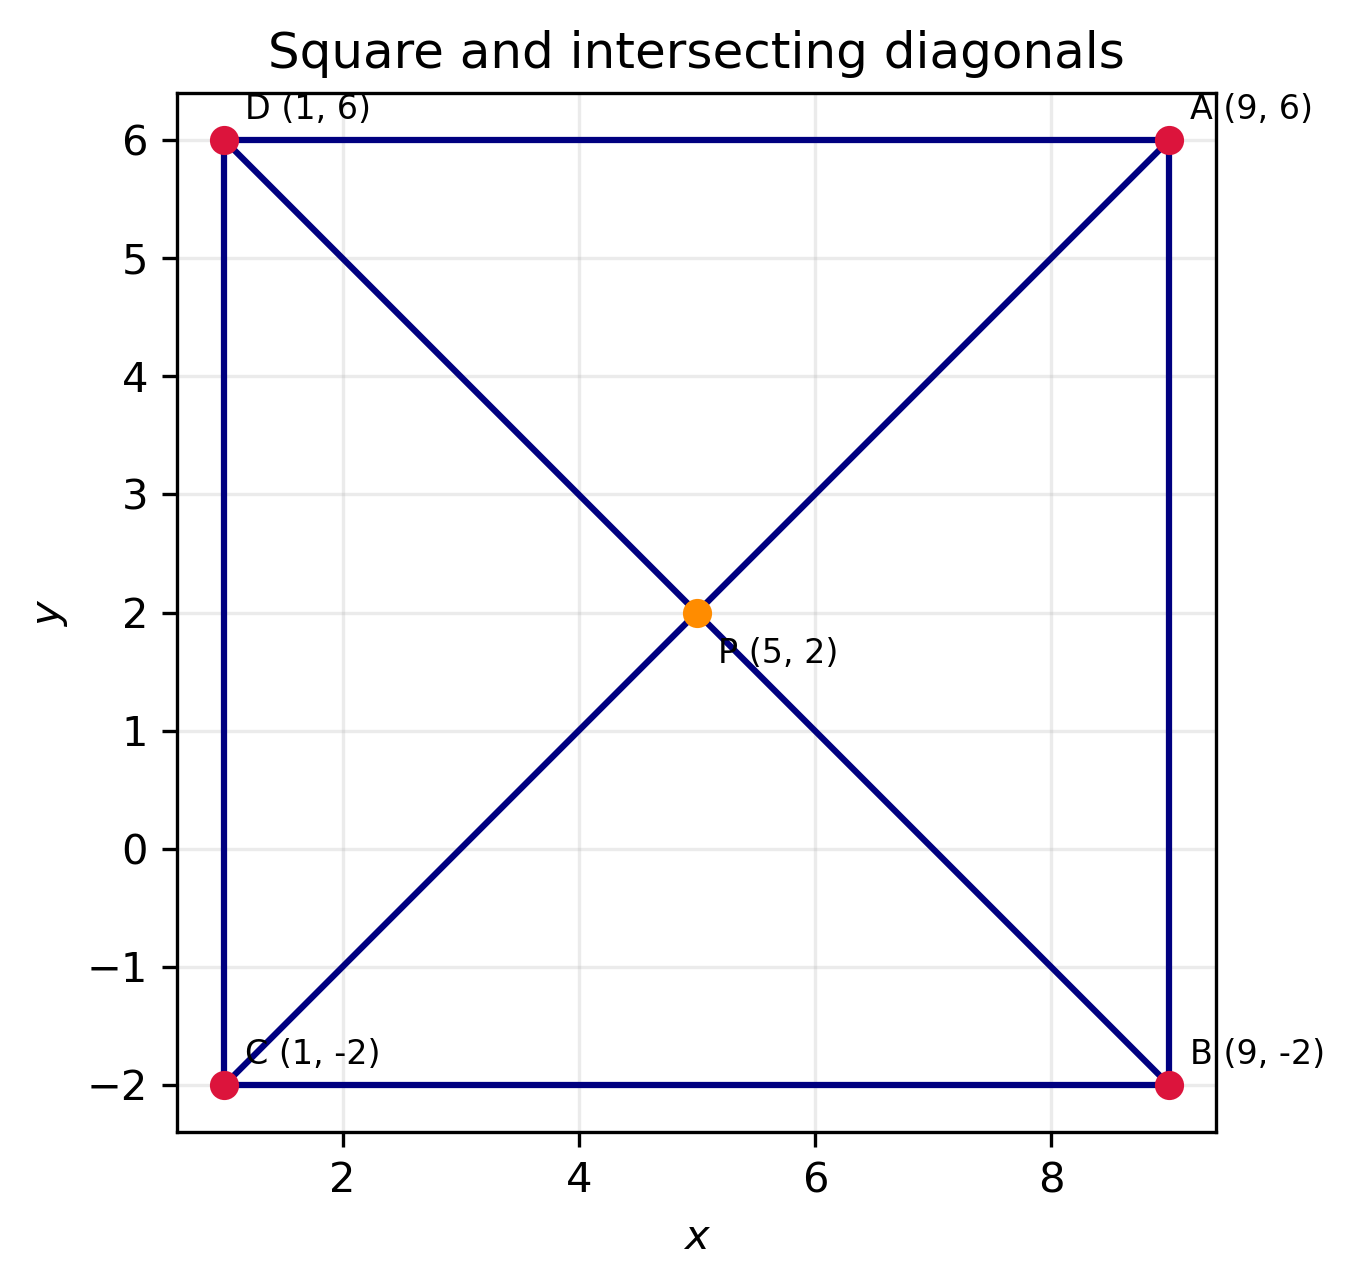
\includegraphics[width=0.49\linewidth]{figs/1.2.10.png}
    \caption{Square $ABCD$ and diagonals meeting at $P$.}
\end{figure}

\item[1.2.11] A chord $AB$ of a circle of radius $7$ cm subtends an angle of $120^\circ$ at the centre. Find (i) the perimeter of major sector $OACB$, and (ii) the area of the shaded segment if $[\triangle OAB]=21.2$ cm$^2$.\nobreak\hfill\mbox{(10,2026)}



\vspace{0.6em}\par\solution


The major arc is $240^\circ$, so the major-sector perimeter is $14+\frac{240}{360}(14\pi)=14+\frac{28\pi}{3}\approx43.32$ cm. The shaded minor segment has area $\frac{120}{360}\pi(7)^2-21.2=\frac{49\pi}{3}-21.2\approx30.11$ cm$^2$. The code draws and shades the segment and calculates both values.
\par\noindent\hfill\mbox{\textit{(\ref{formula-1-1-6})}}\par\begin{lstlisting}[frame=single, basicstyle=\rmfamily, escapeinside={(*@}{@*)}]
(*@\makebox[\dimexpr\linewidth-2\fboxsep-2\fboxrule\relax][c]{codes/1.2.11.py}@*)
\end{lstlisting}
\begin{figure}[H]
    \centering
    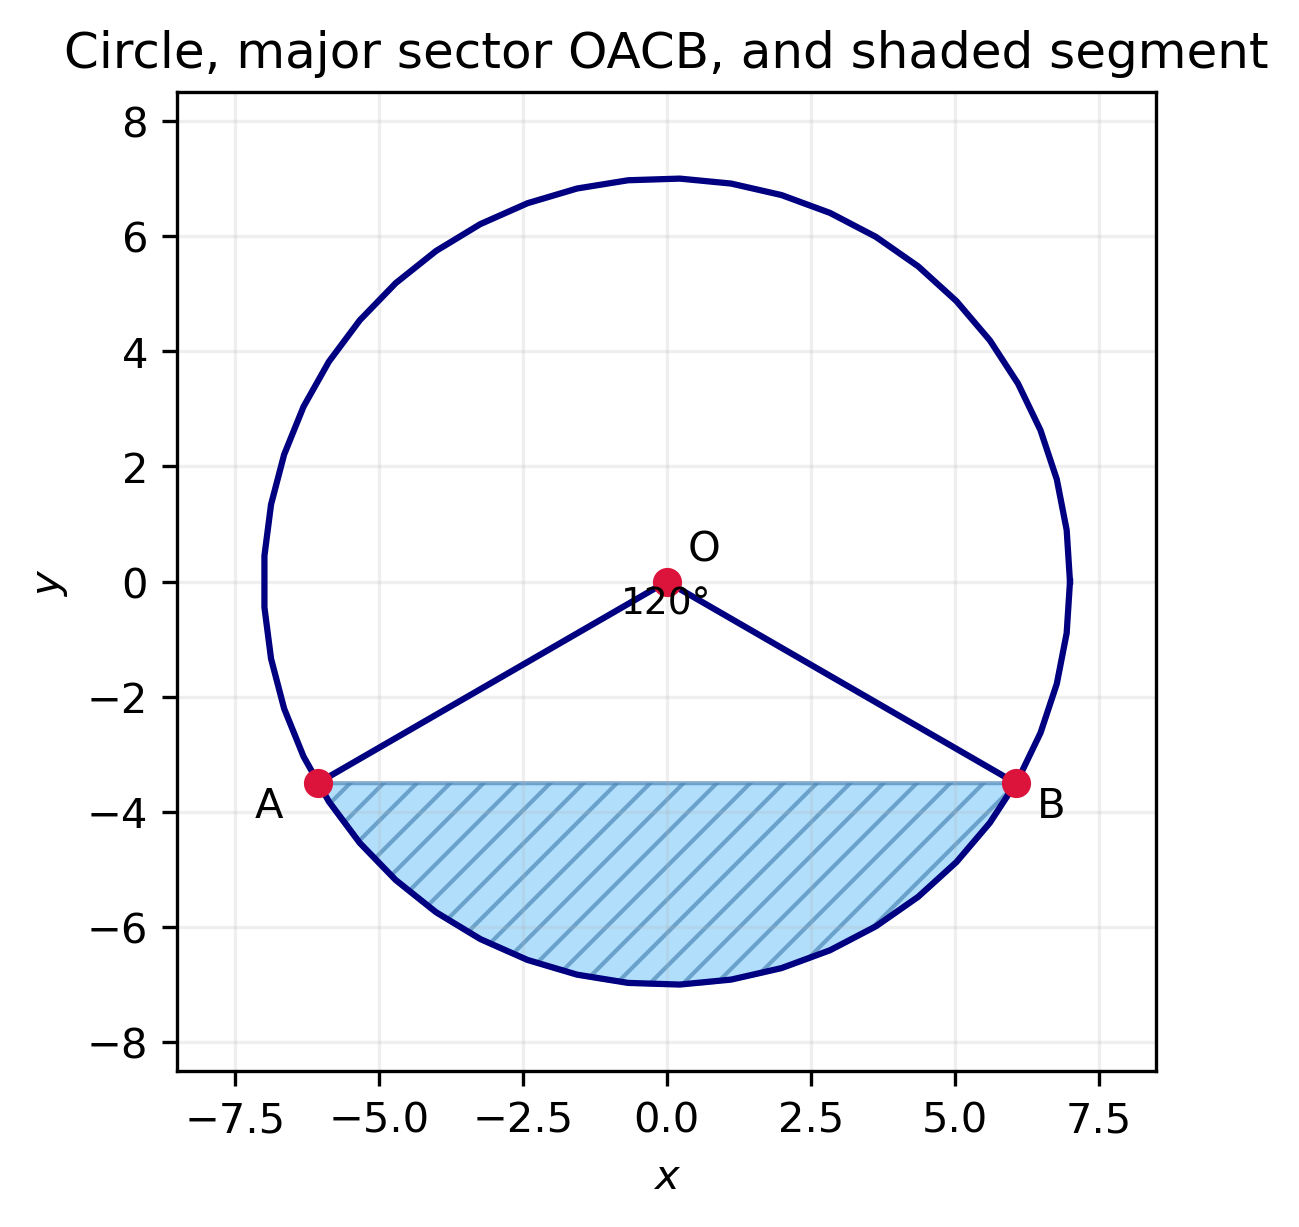
\includegraphics[width=0.47\linewidth]{figs/1.2.11.png}
    \caption{Major sector and shaded minor segment.}
\end{figure}

\item[1.2.12] A point $P(x,7)$ divides the line segment joining $A(-5,4)$ and $B(7,9)$ in a certain ratio. Find the ratio and hence find $x$.\nobreak\hfill\mbox{(10,2026)}



\vspace{0.6em}\par\solution


The vertical changes give $AP:PB=(7-4):(9-7)=3:2$. By the section formula, $x=\frac{3(7)+2(-5)}{3+2}=\frac{11}{5}$. The code plots $A$, $P$, and $B$.
\par\noindent\hfill\mbox{\textit{(\ref{formula-1-1-4})}}\par\begin{lstlisting}[frame=single, basicstyle=\rmfamily, escapeinside={(*@}{@*)}]
(*@\makebox[\dimexpr\linewidth-2\fboxsep-2\fboxrule\relax][c]{codes/1.2.12.py}@*)
\end{lstlisting}
\begin{figure}[H]
    \centering
    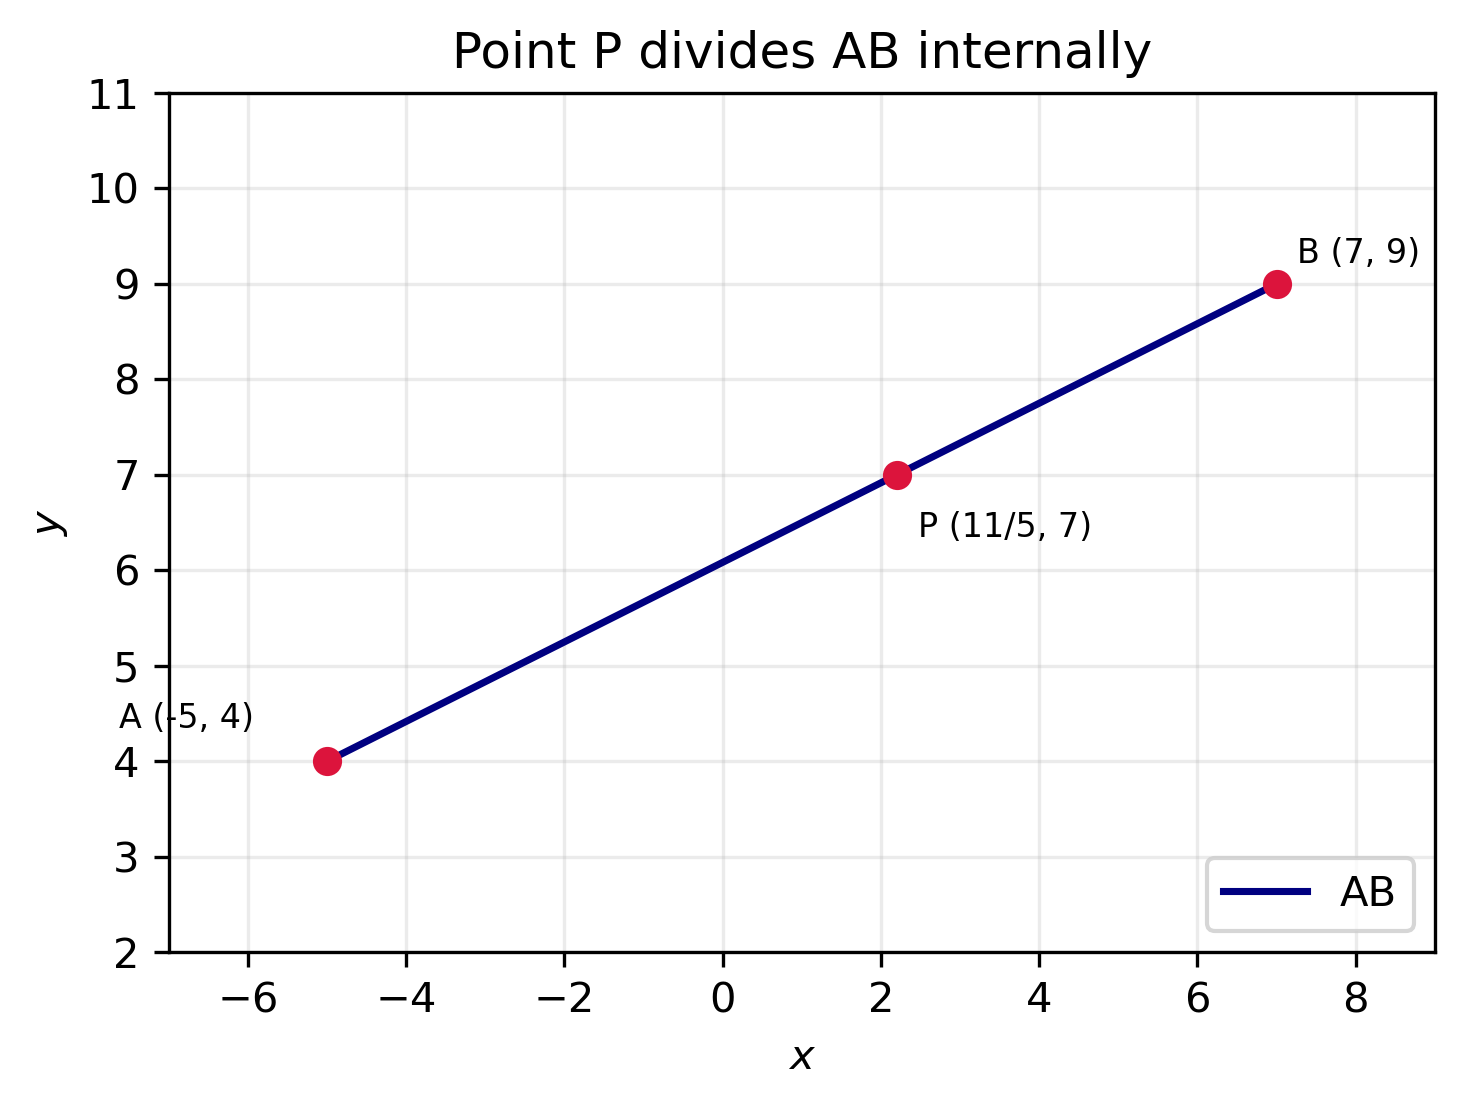
\includegraphics[width=0.52\linewidth]{figs/1.2.12.png}
    \caption{Point $P$ divides $AB$ internally in the ratio $3:2$.}
\end{figure}

\item[1.2.13] In the given figure, $PA$ is tangent to the circle with centre $O$, $OA=10$ cm, $AB=8$ cm, and $AB\perp OP$. Find $PB$.\nobreak\hfill\mbox{(10,2026)}



\vspace{0.6em}\par\solution


In right triangle $OAB$, $OB=\sqrt{10^2-8^2}=6$ cm. Let $PB=t$. Since $PA$ is tangent, $\triangle OAP$ is right-angled at $A$; also $\triangle PAB$ is right-angled at $B$. Thus $t^2+8^2=(t+6)^2-10^2$, giving $t=\frac{32}{3}$ cm. The code constructs this configuration and computes the length.
\par\noindent\hfill\mbox{\textit{(\ref{formula-1-1-2})}}\par\begin{lstlisting}[frame=single, basicstyle=\rmfamily, escapeinside={(*@}{@*)}]
(*@\makebox[\dimexpr\linewidth-2\fboxsep-2\fboxrule\relax][c]{codes/1.2.13.py}@*)
\end{lstlisting}
\begin{figure}[H]
    \centering
    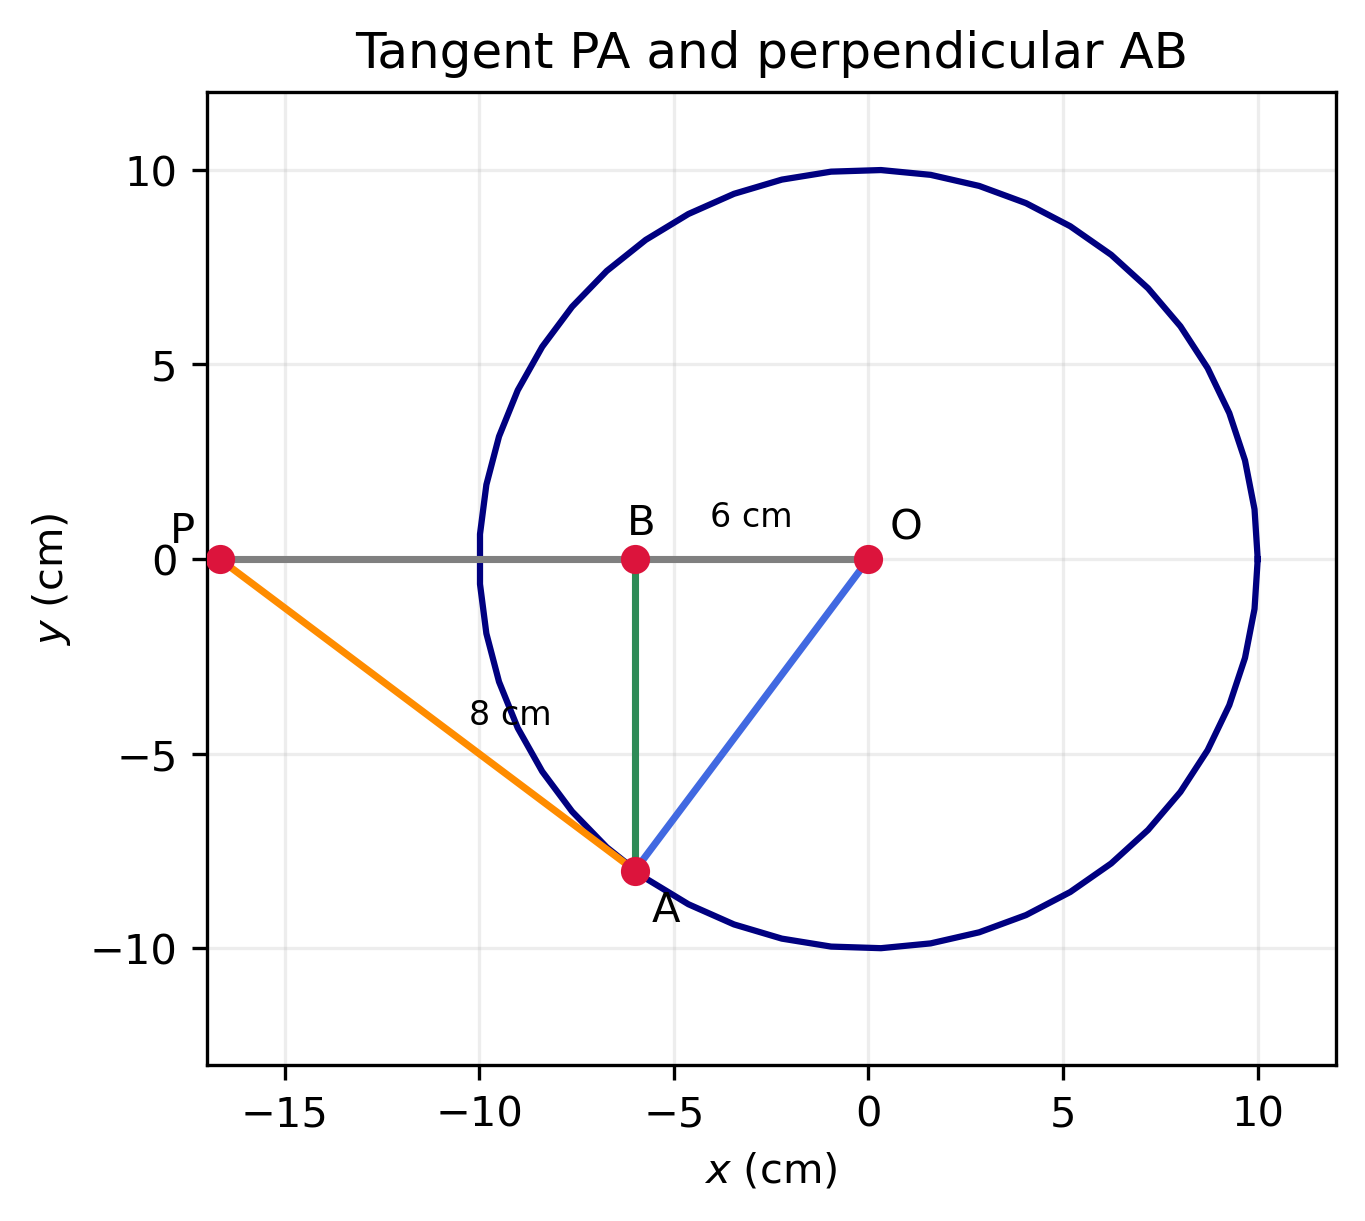
\includegraphics[width=0.50\linewidth]{figs/1.2.13.png}
    \caption{Tangent $PA$ and perpendicular segment $AB$.}
\end{figure}

\item[1.2.14] Solve graphically: $x-2y=3$, $3x-8y=7$.\nobreak\hfill\mbox{(10,2026)}



\vspace{0.6em}\par\solution

The two lines intersect at $(5,1)$, so the solution is $x=5$, $y=1$. The code plots both lines and marks their intersection; it uses the CoordGeo line-intersection function to calculate the point.
\begin{lstlisting}[frame=single, basicstyle=\rmfamily, escapeinside={(*@}{@*)}]
(*@\makebox[\dimexpr\linewidth-2\fboxsep-2\fboxrule\relax][c]{codes/1.2.14.py}@*)
\end{lstlisting}
\begin{figure}[H]
    \centering
    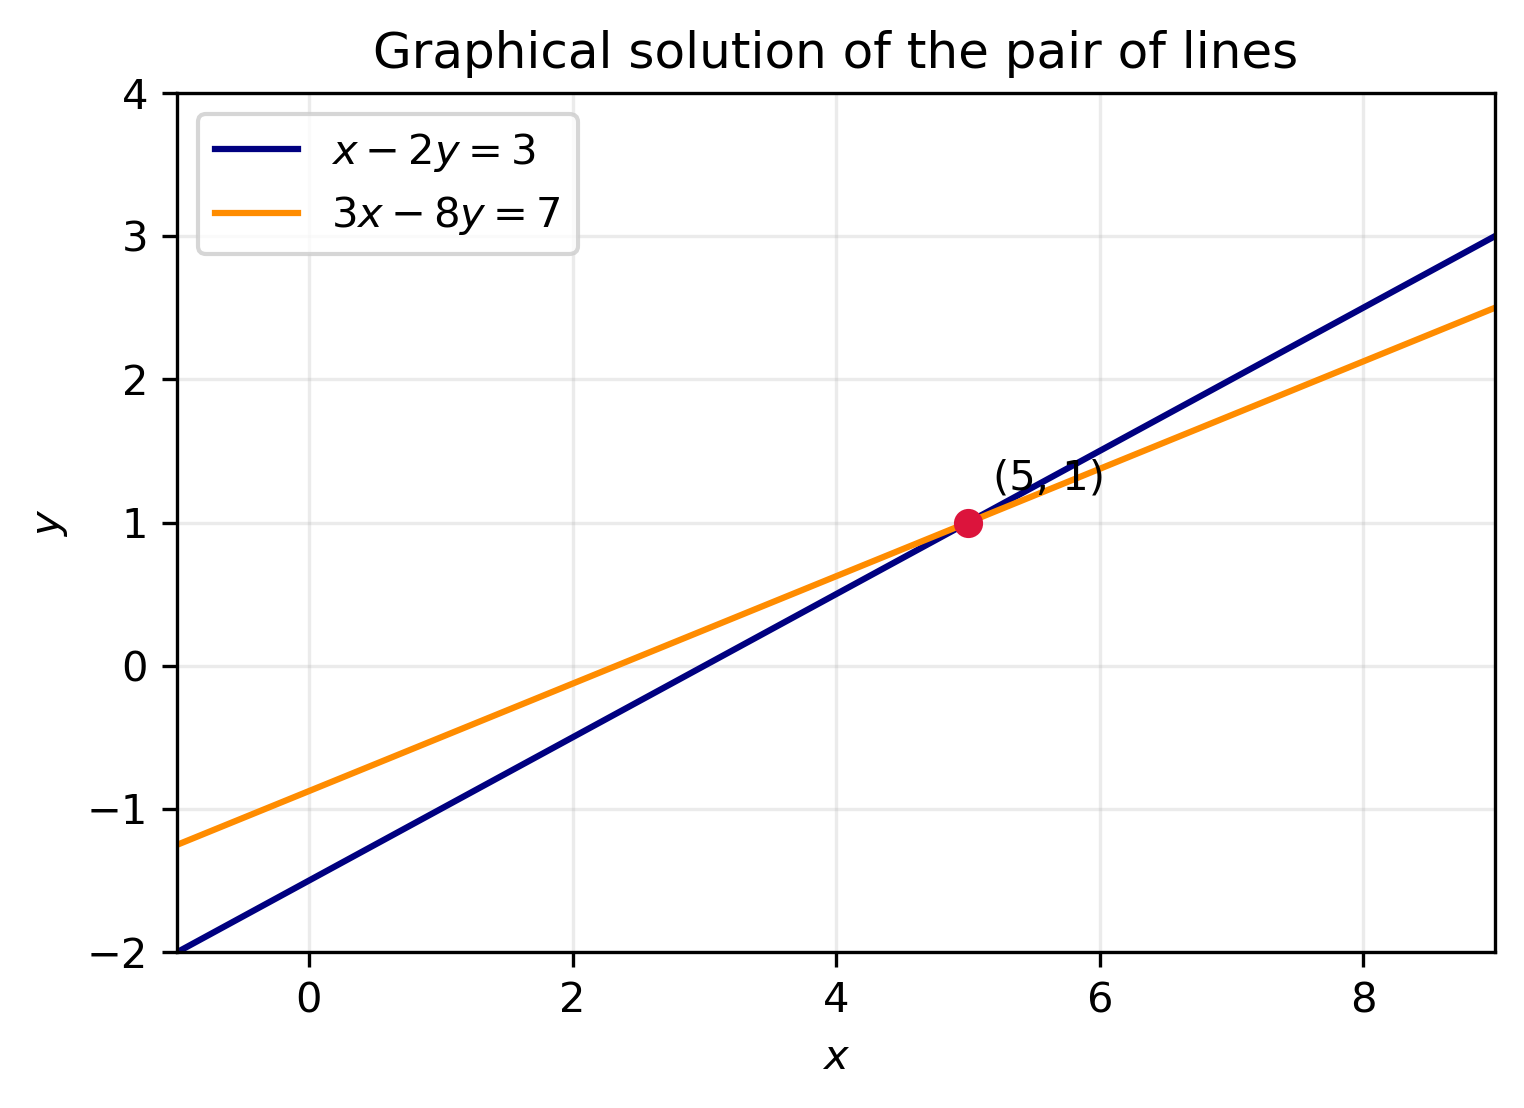
\includegraphics[width=0.52\linewidth]{figs/1.2.14.png}
    \caption{The lines intersect at $(5,1)$.}
\end{figure}

\item[1.2.15] A boy flies a kite with a $60$ m string at an elevation of $30^\circ$. Another boy on the roof of a $20$ m building sees the same kite at $45^\circ$. If the boys are on opposite sides of the kite, find the first boy's distance from the building and the kite's height from the ground. Use $\sqrt3=1.73$.\nobreak\hfill\mbox{(10,2026)}



\vspace{0.6em}\par\solution


Take the first boy as the origin, with horizontal and vertical unit vectors $\mathbf{i}$ and $\mathbf{j}$. The kite's position vector is
\[
\mathbf{k}=60(\cos30^\circ\,\mathbf{i}+\sin30^\circ\,\mathbf{j})=30\sqrt3\,\mathbf{i}+30\,\mathbf{j}.
\]
Thus its height above the ground is $30$ m. The rooftop is $20$ m high, so the kite is $10$ m above it. Since the rooftop boy sees the kite at $45^\circ$ and is on the opposite side, the rooftop position vector is
\[
\mathbf{r}=\mathbf{k}+10\mathbf{i}-10\mathbf{j}=(30\sqrt3+10)\mathbf{i}+20\mathbf{j}.
\]
Subtracting the building's vertical vector $20\mathbf{j}$ gives the building-base position vector $\mathbf{b}=(30\sqrt3+10)\mathbf{i}$. Therefore the first boy's distance from the building is $|\mathbf{b}|=30\sqrt3+10\approx61.9$ m, using $\sqrt3=1.73$. The code plots the configuration.
\par\noindent\hfill\mbox{\textit{(\ref{formula-1-1-7})}}\par\begin{lstlisting}[frame=single, basicstyle=\rmfamily, escapeinside={(*@}{@*)}]
(*@\makebox[\dimexpr\linewidth-2\fboxsep-2\fboxrule\relax][c]{codes/1.2.15.py}@*)
\end{lstlisting}
\begin{figure}[H]
    \centering
    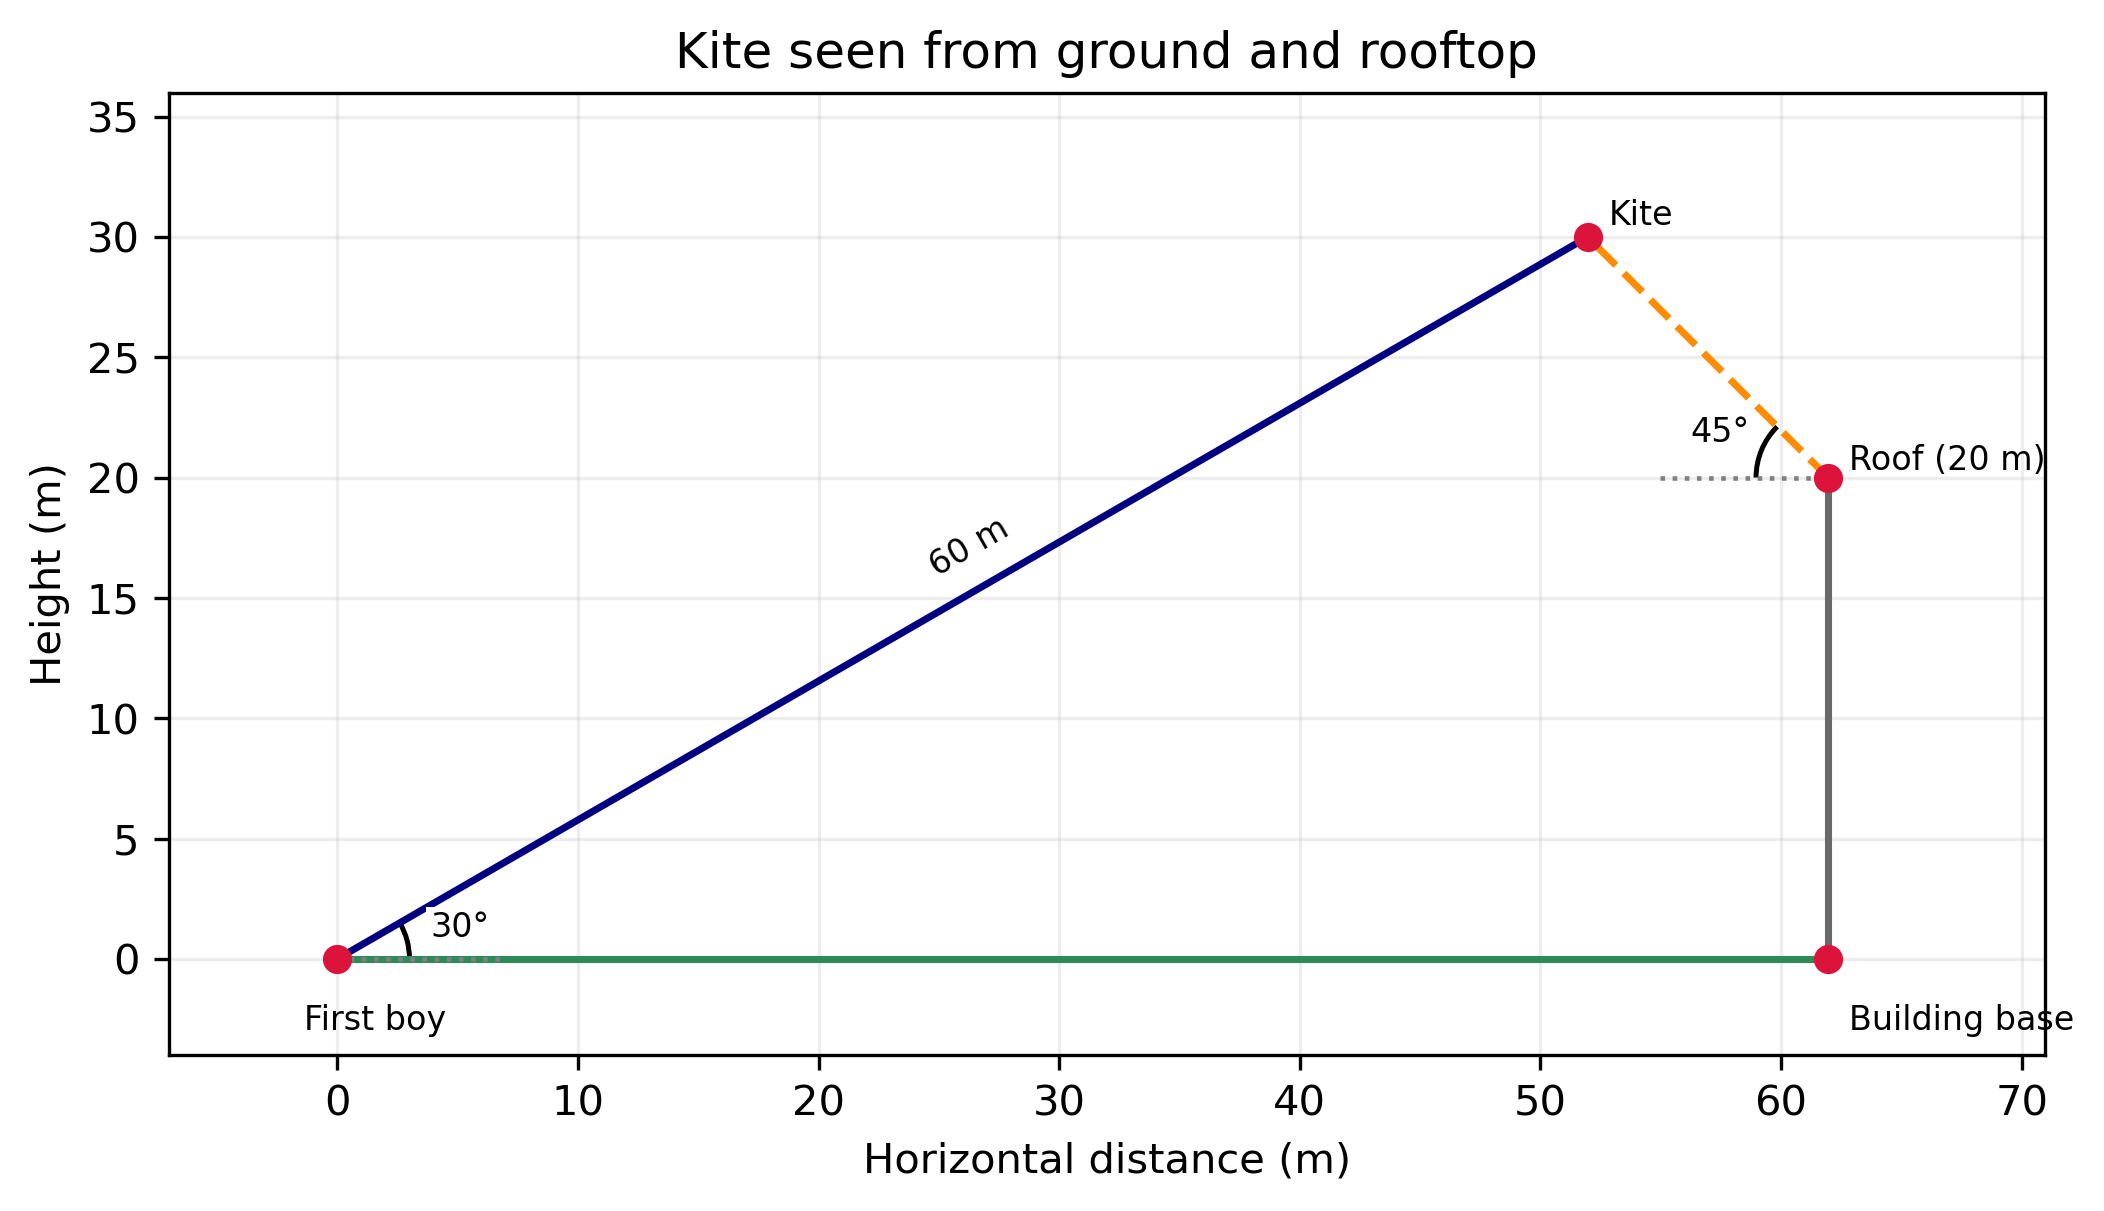
\includegraphics[width=0.58\linewidth]{figs/1.2.15.png}
    \caption{Kite position relative to the two observers.}
\end{figure}

\item[1.2.16] The arch is modelled by $p(x)=-x^2+2x+8$, where $x$ is distance along the stage. Find (i) its height, (ii)(a) its zeroes and the corresponding graph points, or (ii)(b) its span, and (iii) the point where it meets the $y$-axis.\nobreak\hfill\mbox{(10,2026)}



\vspace{0.6em}\par\solution


Writing $p(x)=-(x-1)^2+9$ shows the maximum height is $9$ ft. Factoring gives $p(x)=-(x-4)(x+2)$, so the zeroes are $-2$ and $4$, represented by $(-2,0)$ and $(4,0)$. The span between these intercepts is $6$ ft. At $x=0$, $p(0)=8$, so the $y$-intercept is $(0,8)$.
\par\noindent\hfill\mbox{\textit{(\ref{formula-1-1-1})}}\par
The C program uses Newton--Raphson to find the roots and solve $p'(x)=0$ for the vertex:
\par\noindent\hfill\mbox{\textit{(\ref{formula-1-1-11})}}\par\begin{lstlisting}[frame=single, basicstyle=\rmfamily, escapeinside={(*@}{@*)}]
(*@\makebox[\dimexpr\linewidth-2\fboxsep-2\fboxrule\relax][c]{codes/1.2.16.c}@*)
\end{lstlisting}
The Python program plots the parabola and marks these points:
\begin{lstlisting}[frame=single, basicstyle=\rmfamily, escapeinside={(*@}{@*)}]
(*@\makebox[\dimexpr\linewidth-2\fboxsep-2\fboxrule\relax][c]{codes/1.2.16.py}@*)
\end{lstlisting}
\begin{figure}[H]
    \centering
    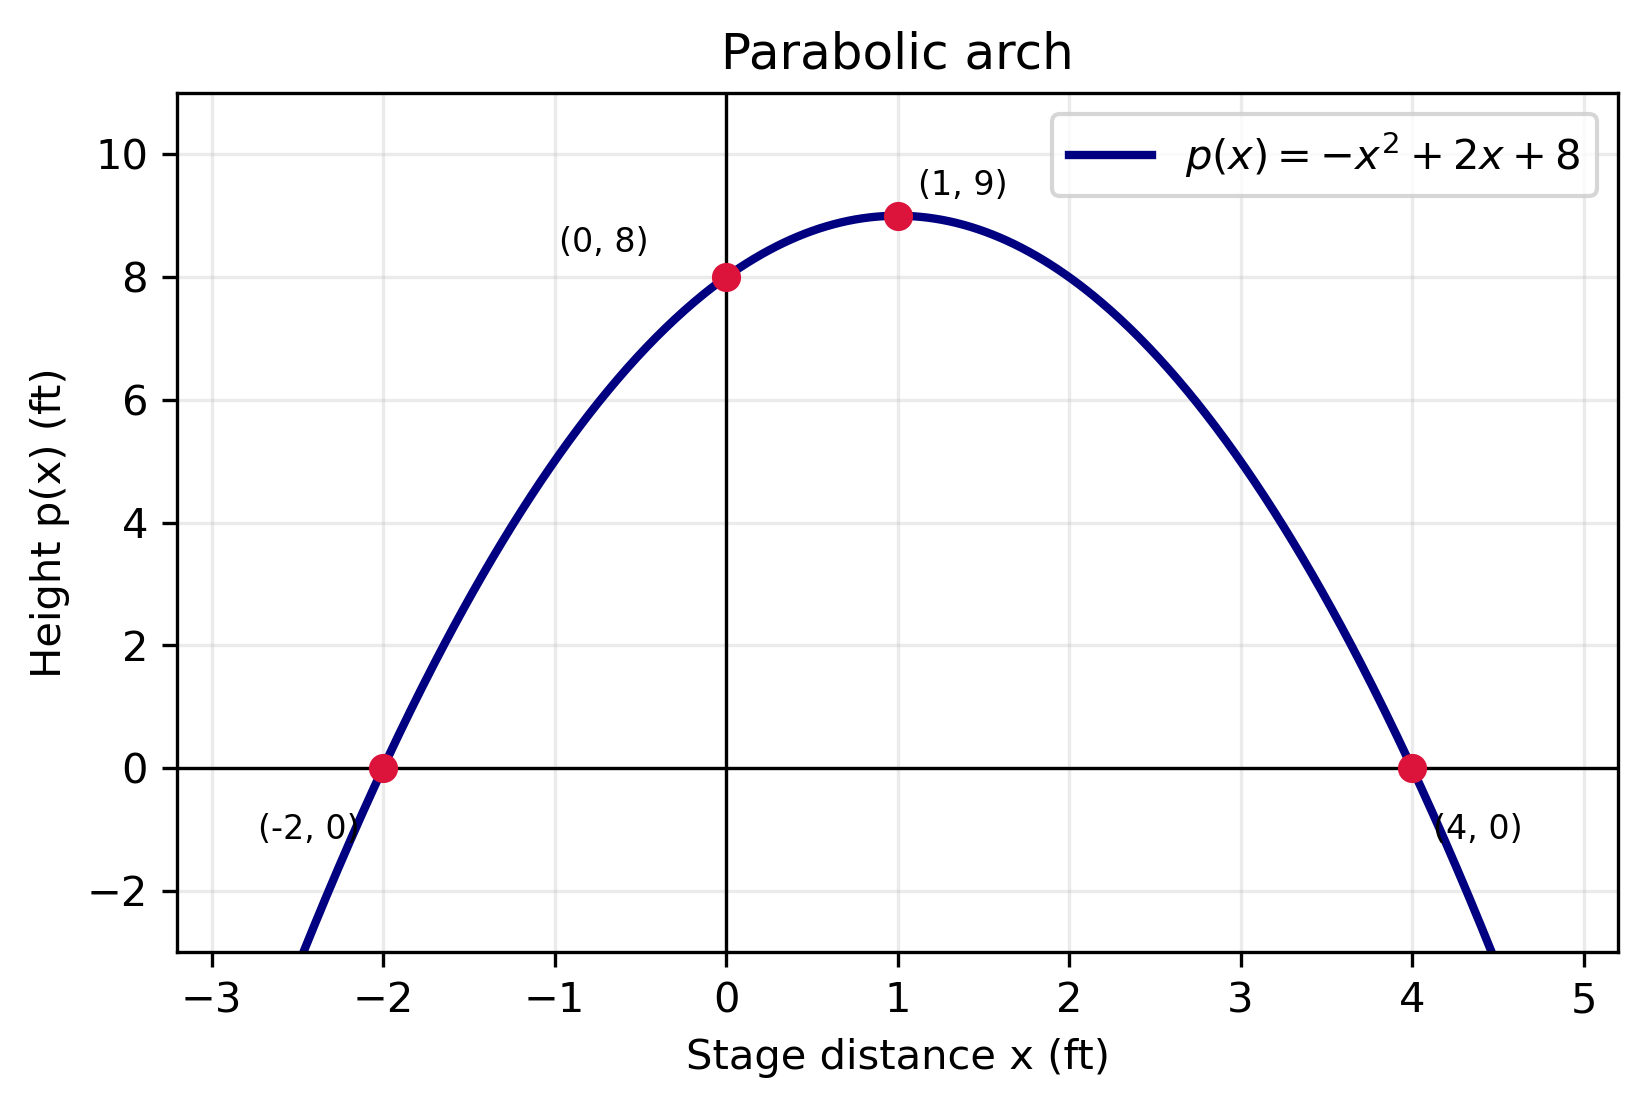
\includegraphics[width=0.56\linewidth]{figs/1.2.16.png}
    \caption{The arch polynomial and its intercepts and vertex.}
\end{figure}

\item[1.2.17] Three cards are dropped from two identical packs: a queen of hearts, a ten of spades, and an ace of clubs. One of the remaining cards is drawn at random. Find (i) the probability of a face card, (ii) the probability of a king or queen, (iii)(a) whether the probability of a queen would be higher if no cards were dropped, or (iii)(b) the probability of a jack and compare it with the probability when no cards were dropped.\nobreak\hfill\mbox{(10,2026)}



\vspace{0.6em}\par\solution


After the drops, $101$ cards remain. Let $X$ be the drawn card's rank category ($K$, $Q$, $J$, or Other). Its PMF with and without the drops is:
\[\begingroup\renewcommand{\arraystretch}{1.25}
\begin{array}{c|cccc}
&K&Q&J&\text{Other}\\\hline
p_X(x)\text{ after drops}&\frac{8}{101}&\frac{7}{101}&\frac{8}{101}&\frac{78}{101}\\
p_X(x)\text{ with no drops}&\frac{8}{104}&\frac{8}{104}&\frac{8}{104}&\frac{80}{104}
\end{array}\endgroup
\]
\par\noindent\hfill\mbox{\textit{(\ref{formula-1-1-9})}}\par
(i) $P(\text{face card})=\frac{8+7+8}{101}=\frac{23}{101}$. (ii) $P(K\text{ or }Q)=\frac{8+7}{101}=\frac{15}{101}$.

(iii)(a) $\frac{7}{101}<\frac{8}{104}$, so queens are more likely with no drops. (iii)(b) $\frac{8}{101}>\frac{8}{104}$; since no jack was removed, jacks are more likely after the drops.

\end{enumerate}
